\chapter[Activity Code]{Activity Code: Design and Implementation}

\begin{changemargin}{1.0cm}{1.0cm}
\abstractpreamble{A computer program was developed to calculate the radioactivity of an ion irradiated target.  The code has been released in two versions, with the first being written in Fortran and the second in Python.  \acrshort{srim}, an ion transport code, was used to calculate proton trajectories used by the Activity codes.\\
\\
Decay equations were derived to calculate the activity of isotopes within the target at time t during and after irradiation.  These were created in a similar manner to the Bateman equations for radioactive decay, but include source terms and branching factors for radioactive isotopes in a decay chain.  These were implemented in a module and class for each version of the code.\\
\\
The University of Birmingham cyclotron was used to activate Iron samples (this work) and Molybdenum (a colleagues work).  The radioactivity of these samples were compared to the predicted activity and gamma lines of the Activity code.\\
\\
Finally, the latest version of the Activity code was used to predict the activity of a Steel specified by another colleague and a set of Iron samples irradiated to 100DPA at varying proton energies.  The results of these simulations are presented in this chapter.
}
\end{changemargin}



\section{Introduction}


High flux neutron reactors are expensive to use, whereas proton accelerators capable of producing beams of adequate fluence and energy are more readily available, cheaper to buy and cheaper to run.  Ion beams, due to the Coulomb interaction, are more controllable in terms of energy, direction and fluence.  They may be concentrated on a desired target at a set fluence and energy.

Depending on the energy of the ion beam, the target material will become radioactive.  The stable nuclei are transmuted and when the resulting isotope is unstable it will decay.  An equation was derived to predict the activity of isotopes for any decay chain with source terms and branching factors included.  Two versions of a computer code were developed to compute the reaction rates and activity of the irradiated targets.



%%====================================================================================================================================================
%%
%%  Part 2: Activity Code
%%
%%====================================================================================================================================================

\section{Activation by Ion Irradiation}



The Bateman equation was derived using Laplace transforms, and this same method has been used to develop a modified equation that incorporates branching factors and production rates for each isotope in the decay chain, as illustrated by figure \ref{fig:decaytree}.

\begin{figure}[!h]
	\centering
	\begin{tikzpicture}[node distance=2cm]
	% Row 1
	\node (parent) [startstop] {Parent Isotope};
	\node (parent_source) [process, left of=parent, xshift=-4cm] {Parent Source};
	% Row 2
	\node (parent_branch) [decision, below of=parent] {Branching};
	% Row 3
	\node (daughter_1a) [process, below of=parent_branch, xshift=-2.5cm] {Daughter 1 (Branch A)};
	\node (daughter_1a_src) [process, left of=daughter_1a, xshift=-2.5cm] {External Source};
	\node (daughter_1b) [process, below of=parent_branch, xshift=2.5cm] {Daughter 1 (Branch B)};
	\node (daughter_1b_src) [process, right of=daughter_1b, xshift=2.5cm] {External Source};
	% Row 4
	\node (daughter_1a_branch) [decision, below of=daughter_1a, xshift=0.5cm] {Branching};
	% Row 5
	\node (daughter_2a) [process, below of=daughter_1a_branch, xshift=-0.5cm] {Daughter 2 (Branch A)};
	\node (daughter_2a_src) [process, left of=daughter_2a, xshift=-2.5cm] {External Source};
	\node (daughter_2b) [process, below of=daughter_1a_branch, xshift=4.5cm] {Daughter 2 (Branch B)};
	\node (daughter_2b_src) [process, right of=daughter_2b, xshift=2.5cm] {External Source};
	
	% arrows
	\draw [thick,->] (parent_source) -- (parent);
	\draw [thick,->] (parent) -- (parent_branch);
	\draw [thick,->] (parent_branch) -- (daughter_1a);
	\draw [thick,->] (parent_branch) -- (daughter_1b);
	\draw [thick,->] (daughter_1a_src) -- (daughter_1a);
	\draw [thick,->] (daughter_1b_src) -- (daughter_1b);
	\draw [thick,->] (daughter_1a) -- (daughter_1a_branch);
	\draw [thick,->] (daughter_1a_branch) -- (daughter_2a);
	\draw [thick,->] (daughter_1a_branch) -- (daughter_2b);
	\draw [thick,->] (daughter_2a_src) -- (daughter_2a);
	\draw [thick,->] (daughter_2b_src) -- (daughter_2b);
	
	%\draw [->] (isotope1) -- (isotope2);
	%\draw [->] (isotope2) -- (stable);
	\end{tikzpicture}
	\captionsetup{font={it}}
	\caption{An example of several decay chains including branching factors and possible external source terms for each isotope on each chain.}
	\label{fig:decaytree}
\end{figure}


\subsection{Laplace Transform}
\label{section:laplaceequations}

Laplace Transforms (eq. \ref{eq:eqLaplaceTransform}) are a useful mathematical tool, and allow ordinary differential equations to be solved by simple algebraic manipulation in the s domain (appendix \ref{chapter:usefullaplacetransforms}).  Bateman took advantage of Laplace Transforms in deriving his equation, and this is the method that has been taken here as well.

\eqLaplaceTransform


\subsection{Constructing the Differential Equations}

The first step is to set up differential equations for the parent isotope, unstable daughter isotopes and stable daughter isotope.  The parent isotope has a source term, due to production, and a loss term, due to decay.  The unstable daughter isotopes have two source terms, from the production by irradiation induced transmutation and the decay of preceding isotopes in the decay chain, and a loss term, due to decay.  Finally, the stable daughter that finalizes the decay chain has two source terms (the same as the unstable daughters) but no loss term.

The variables (and vectors) used in these equations are defined as follows:
\begin{itemize}
	\item $\vec{\lambda}$  vector containing isotope decay constants $\lambda_i$
	\item $\vec{b}$  vector containing isotope to isotope branching factors $b_i$
	\item $\vec{w}$  vector containing isotope production rates $w_i$
	\item $t$  time at which activity/amount of isotope is measured
	\item $N_{i}(0)$ starting amount of the i\textsuperscript{th} isotope
	\item $N_{i}(t)$ amount of the i\textsuperscript{th} isotope at time t
	\item $N'_{i}(t)$ change in amount of the i\textsuperscript{th} isotope, with respect to time, at time t
\end{itemize}

The differential equations for the parent isotope (first isotope), unstable daughter isotopes (i\textsuperscript{th} isotopes) and stable, final, daughter isotope (zth isotope) in the time domain are as follows:

\begin{equation}
N'_{1}(t) = \omega_{1} - \lambda_{1} N_{1} (t)
\end{equation}

\begin{equation}
N'_{i}(t) = \omega_{i} + b_{i-1} \lambda_{i-1} N_{i-1} (t) - \lambda_{i} N_{i} (t)
\end{equation}

\begin{equation}
N'_{z}(t) =  \omega_{z} + b_{z-1} \lambda_{z-1} N_{z-1} (t)
\end{equation}

Applying the Laplace Transform to these three differential equations allows them to be manipulated and solved algebraically in the s-domain.

\begin{equation}
N_{1}(s) = \frac{1}{s+\lambda_{1}} N_{1}(0) + \frac{1}{s(s+\lambda_{1})} \omega_{1}
\end{equation}

\begin{equation}
N_{i}(s) = \frac{1}{s ( s+ \lambda_{i})} \left(\omega_{i} \right) + \frac{1}{s+ \lambda_{i}} \left( b_{i-1} \lambda_{i-1} N_{i-1} (s) \right) + \frac{1}{s+ \lambda_{i}} N_{i} (0)
\end{equation}

\begin{equation}
N_{z}(s) = \frac{1}{s^2} \omega_{z} + \frac{1}{s} b_{z-1} \lambda_{z-1} N_{z-1} (s) + \frac{1}{s} N_{z}(0)
\end{equation}


\subsection{Numerical Inversion of the Laplace Transform}

The Gaver-Stehfest\cite{stehfest} algorithm was developed in the 1960s and 1970s and is a method of calculating the inverse of a Laplace Transform in the real number domain.  It is an easy to implement and reasonably accurate method, although it is an approximation to the real value.  A comparison between an analytic and numeric inversion for the unstable isotope Po-218 is discussed at the end of this section (figure \ref{fig:po218decay}).

\begin{equation}
f(t) \approx f_{n}(t) = \frac{\ln(2)}{t} \sum_{k=1}^{2n} a_{k}(n)F(s) \textnormal{ where } n \ge 1, t>0
\end{equation}

\begin{equation}
s = \frac{k \ln(2)}{t}
\end{equation}

\begin{equation}
a_{k}(n) = \frac{(-1)^{(n+k)}}{n!} \sum_{j=Floor(\frac{k+1}{2})} j^{n+1} \left( \begin{matrix} n \\ j \end{matrix} \right)  \left( \begin{matrix} 2j \\ j \end{matrix} \right)  \left( \begin{matrix} j \\ k-j \end{matrix} \right)
\end{equation}

The equation for the i\textsuperscript{th} isotope may be calculated by recursively calculating the equations by numeric inversion, starting from the first (parent isotope) and inserting the result into each subsequent recursion until the i\textsuperscript{th} isotope is reached (changing the equations appropriately for the parent, unstable daughter and stable daughter isotopes).


\subsection{Analytic Solution by Partial Fraction Expansion}
\label{section:activitysolution}

The equation for the i\textsuperscript{th} isotope in the s domain can be written in full by substituting the preceding equation until the parent isotope is reached, and this full equation may be rearranged with the production amount of each isotope and starting amount of each isotope in individual terms.  Each of these terms is multiplied by a fraction that can be expanded, using partial fractions, and inverted analytically.

This is illustrated with an example unstable isotope, fourth in the decay chain (including the parent isotope) (eq. \ref{eq:example4thchainunstable}).

\begin{equation}
\begin{split}
N_{4}(s) =
\frac{1}{(s+\lambda_1)(s+\lambda_2)(s+\lambda_3)(s+\lambda_4)} b_{2} b_{3} b_{4} \lambda_1 \lambda_2 \lambda_3 N_{1}(0) \\
+ \frac{1}{(s+\lambda_2)(s+\lambda_3)(s+\lambda_4)} b_{3} b_{4} \lambda_2 \lambda_3 N_{2}(0) \\
+ \frac{1}{(s+\lambda_3)(s+\lambda_4)} b_{4} \lambda_3 N_{3}(0) \\
+ \frac{1}{(s+\lambda_4)} N_{4}(0) \\
+ \frac{1}{s(s+\lambda_1)(s+\lambda_2)(s+\lambda_3)(s+\lambda_4)} b_{2} b_{3} b_{4} \lambda_1 \lambda_2 \lambda_3 \omega_{1} \\
+ \frac{1}{s(s+\lambda_2)(s+\lambda_3)(s+\lambda_4)} b_{3} b_{4} \lambda_2 \lambda_3 \omega_{2} \\
+ \frac{1}{s(s+\lambda_3)(s+\lambda_4)} b_{4} \lambda_3 \omega_{3} \\
+ \frac{1}{s(s+\lambda_4)} \omega_{4}
\end{split}
\label{eq:example4thchainunstable}
\end{equation}

An example stable isotope, fourth (last) in the decay chain (including the parent isotope) (eq. \ref{eq:example4thchainstable}).

\begin{equation}
\begin{split}
N_{4}(s) =
\frac{1}{s(s+\lambda_1)(s+\lambda_2)(s+\lambda_3)} b_{2} b_{3} b_{4} \lambda_1 \lambda_2 \lambda_3 N_{1}(0) \\
+ \frac{1}{s(s+\lambda_2)(s+\lambda_3)} b_{3} b_{4} \lambda_2 \lambda_3 N_{2}(0) \\
+ \frac{1}{s(s+\lambda_3)} b_{4} \lambda_3 N_{3}(0) \\
+ N_{4}(0) \\
+ \frac{1}{s^2(s+\lambda_1)(s+\lambda_2)(s+\lambda_3)} b_{2} b_{3} b_{4} \lambda_1 \lambda_2 \lambda_3 \omega_{1} \\
+ \frac{1}{s^2(s+\lambda_2)(s+\lambda_3)} b_{3} b_{4} \lambda_2 \lambda_3 \omega_{2} \\
+ \frac{1}{s^2(s+\lambda_3)} b_{4} \lambda_3 \omega_{3} \\
+ \frac{1}{s^2} \omega_{4}
\end{split}
\label{eq:example4thchainstable}
\end{equation}

By using partial fraction expansion and standard Laplace Transforms, the set of equations (eqs. \ref{eq:unstable1}, \ref{eq:unstable2}, \ref{eq:unstable3}, \ref{eq:unstable4}) is used to calculate the amount of the m\textsuperscript{th} isotope in the decay chain, providing the m\textsuperscript{th} isotope is unstable.

\begin{equation}
\begin{split}
N_{m}(t; \vec{\lambda}, \vec{b}, \vec{w}, \vec{N_{0}})
= \sum_{k=1,m} r(k, m, \vec{\lambda}, \vec{b}) \left[ f(t; k,m,\vec{\lambda}) N_{0, k} + g(t;k,m,\vec{\lambda}) w_{k} \right ]
\end{split}
\label{eq:unstable1}
\end{equation}

\begin{equation}
\begin{split}
r(k,m,\vec{\lambda}, \vec{b}) =
\begin{cases}
\prod_{i=k,m-1} \left( b_{i+1} \lambda_{i} \right) , & \text{if } k < m\\
1, & \text{if }k = m
\end{cases}
\end{split}
\label{eq:unstable2}
\end{equation}

\begin{equation}
\begin{split}
f(t;k,m,\vec{\lambda})
=
(-1)^{m-k}
\sum_{i=k,m}
\left[
\frac{\exp(-\lambda_i t)}{\prod_{j=k,m;j\neq i}\left(\lambda_i-\lambda_j\right )}
\right ]
\end{split}
\label{eq:unstable3}
\end{equation}

\begin{equation}
\begin{split}
g(t;k,m,\vec{\lambda})
= \frac{1}{\prod_{i=k,m} \lambda_i }
+ \left( -1 \right)^{m-k+1}
\sum_{i=k,m}
\left[
\frac{\exp(-\lambda_i t)}{\lambda_i \prod_{j=k,m;j\neq i}\left(\lambda_i - \lambda_j\right )}
\right]
\end{split}
\label{eq:unstable4}
\end{equation}

The set of equations (eqs. \ref{eq:stable1}, \ref{eq:stable2}, \ref{eq:stable3}, \ref{eq:stable4}) is used to calculate the amount of the m\textsuperscript{th} isotope in the decay chain, where the m\textsuperscript{th} isotope is stable.

\begin{equation}
\begin{split}
N_{m}(t; \vec{\lambda}, \vec{b}, \vec{w}, \vec{N_{0}})
= N_{m} + w_{m} t +
\sum_{k=1,m-1} r(k, m, \vec{\lambda}, \vec{b}) \left[ f(t; k,m-1,\vec{\lambda}) N_{0,k} + g(t;k,m,\vec{\lambda}) w_{k} \right ]
\end{split}
\label{eq:stable1}
\end{equation}

\begin{equation}
\begin{split}
r(k,m,\vec{\lambda}, \vec{b}) =
\begin{cases}
\prod_{i=k,m-1} \left( b_{i+1} \lambda_{i} \right) , & \text{if } k < m\\
1, & \text{if }k = m
\end{cases}
\end{split}
\label{eq:stable2}
\end{equation}

\begin{equation}
\begin{split}
f(t;k,m,\vec{\lambda})
= \frac{1}{\prod_{i=k,m-1} \lambda_i }
+ \left( -1 \right)^{m-k+1}
\sum_{i=k,m-1}
\left[
\frac{\exp(-\lambda_i t)}{\lambda_i \prod_{j=k,m-1;j\neq i}
\left({\lambda_i - \lambda_j}
\right )}
\right]
\end{split}
\label{eq:stable3}
\end{equation}

\begin{equation}
\begin{split}
g(t;k,m,\vec{\lambda})
= \frac{1}{\prod_{i=k,m-1} \lambda_i } t
- \frac{\sum_{i=k,m-1} \left[ \prod_{j=k,m-1; j \neq i} \lambda_{j} \right]}
{\prod_{i=k,m-1} \lambda_{i}^2}
+ \left( -1 \right)^{m-k+1}
\sum_{i=k,m-1}
\left[
\frac{\exp(-\lambda_i t)}{\lambda_i^2 \prod_{j=k,m-1;j\neq i}\left(
\lambda_i - \lambda_j \right)}
\right]
\end{split}
\label{eq:stable4}
\end{equation}

\subsection{Preference: Analytic over Numeric}

\begin{figure}
	\begin{center}
		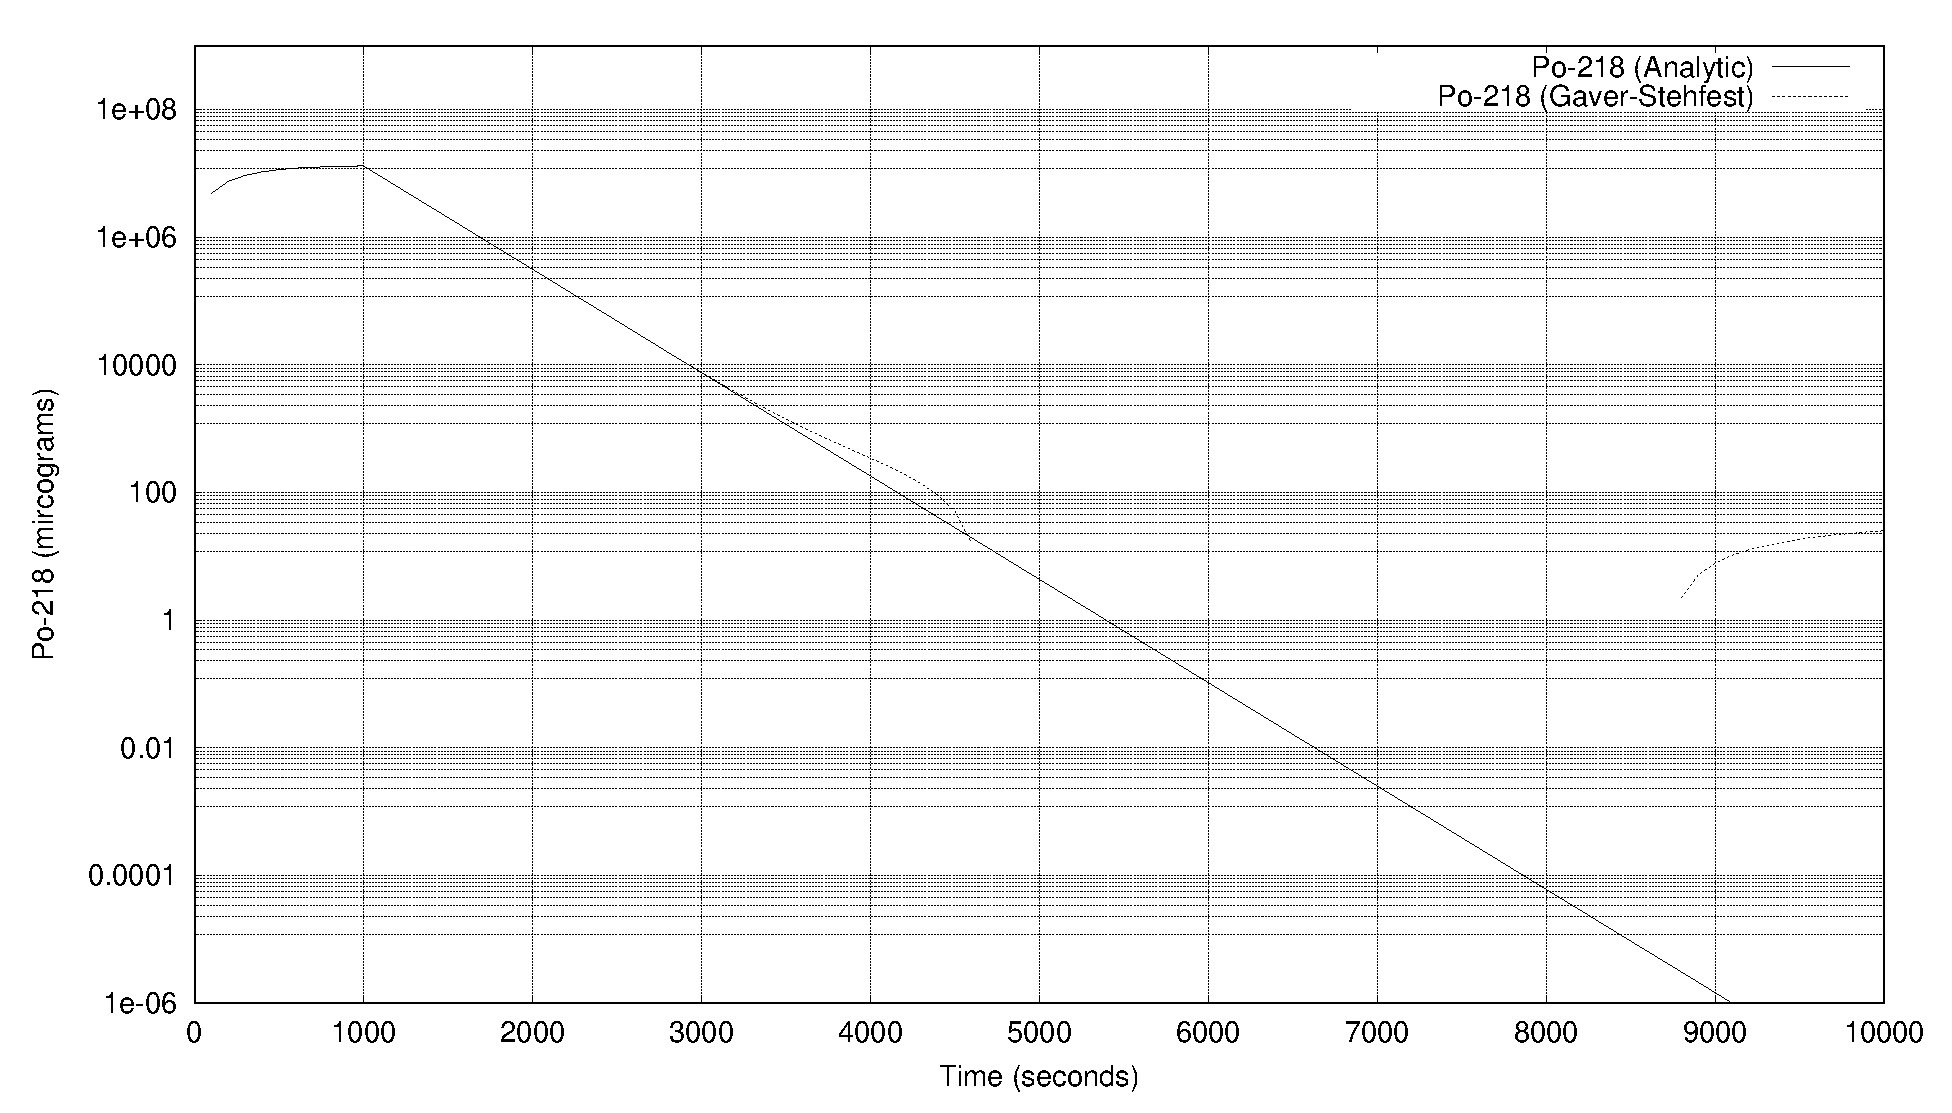
\includegraphics[width=15.0cm]{chapters/activity_code/plots/po-218/po218_po218.eps}
		\captionsetup{font={it}}
		\caption{Decay of Po-218: Analytic and Gaver-Stehfest Calculations \cite{jeff311}}
		\label{fig:po218decay}
	\end{center}
\end{figure}

The numeric solution only requires the equation to be solved in the s-domain; the Gaver-Stehfest algorithm performs the inversion.  It is worth the extra effort to derive and implement an analytic solution, as the numeric is only an approximation.  Examples of the pitfalls of the numeric solution are that it can give negative amounts of an isotope and the difference between the numeric and analytic calculated amounts can become quite large when the isotope decays away to a very small value.  Figure \ref{fig:po218decay} shows the predicted decay of a sample of Po-218 irradiated for 1,000s, and sampled until 10,000s.  In the region between 4,000s and 9,000s the amount from the numeric calculation drops below zero, whereas the analytic calculation remains above zero, as would be expected.



\FloatBarrier
\section{Activity Code}

The first version of the Activity code was written in Fortran.  A paper that describes this code is contained in section \ref{section:activityv1published} of the appendix along with the manual describing how to use it (section \ref{section:activityv1published}).  This version used the TENDL-2013 cross section database and was replaced by a version of the code written in Python.

There were a number of issues with version 1 of the computer code.  It was written in Fortran, but over time this has been a stumbling block for new users, especially those new to Linux and unfamiliar with Fortran. 

In the first version of the code, the trajectory data was replaced with a series of polynomials, but this method was not a reliable solution and it was preferred to use the data directly to calculate the reaction rates.  Finally, a language such as Python3 is more widely used and contains very useful features such as dictionaries and a plotting module (matplotlib).


\subsection{Computer Code Development}

Activity V2 uses a custom cross section database generated using the TALYS nuclear reaction code along with the JEFF3.1.1 datafile for decay data.  All the data has been processed and is packaged with the source code.  The source code and instructions on how to use the program are available to download from GitHub: 

https://github.com/BenPalmer1983/activity\_v2

As with version 1, the user provides an ion trajectory file and an input file that specifies beam parameters and target composition.  The code may be used for both protons and deuterons, providing the correct trajectory file has been generated.  It does also contain neutron reaction cross sections and may be used for very thin foils with a flat distribution of neutron energies.




\subsection{Extended Bateman Equations}

The Bateman equations were derived from scratch to include a source term for each isotope and branching factors from parent isotope to daughter isotope(s).  This process along with the numerical and analytic solutions are outlined in section \ref{section:activitysolution}.

\FloatBarrier

The decay equations were programmed as a class in python (appendix \ref{section:decayclass}) that used decay data accessible through a second class, isotopes, populated with data from the JEFF 3.1.1 data file.  The static function for computing activity in this class was tested against numerically computed values.  

\begin{figure}[h]
  \begin{center}
    
\includegraphics[width=0.7\linewidth]{chapters/activity_code/84po216/84Po216_path.png}
    \caption{Decay path of Polonium-216}
    \label{fig:DecayPathPo216}
  \end{center}
\end{figure}

Due to the large range in magnitude of the half life for various isotopes, a decay chain was selected where the time step for the numeric calculation would be applicable to the half life of the isotopes in the decay chain, whilst keeping the number of steps low enough to compute the activities in a reasonable amount of time with a simple algorithm.  The decay path of  ${}^{216}_{84}Po$ (figure \ref{fig:DecayPathPo216}) contains 6 isotopes and includes one branch at ${}^{212}_{83}Bi$.

\begin{table}[h]
\begin{center}
\begin{tabular}{c c}
\hline\hline
Isotope & Half Life (s)\\
\hline\hline
Po-216 & $1.45 \times 10^{-1}$ \\
Pb-212 & $3.83 \times 10^{4}$ \\
Bi-212 & $3.63 \times 10^{3}$ \\
Po-212 & $2.99 \times 10^{-7}$ \\
Tl-212 & $3.1 \times 10^{1}$ \\
Pb-208 & Stable \\
\hline\hline
\end{tabular}
\end{center}
\caption{Half life of isotopes in the Po-216 decay chain}
\label{table:po216halflives}
\end{table}

The range of half life times (table \ref{table:po216halflives}) in the Polonium decay chain was from $3.83 \times 10^4$s for ${}^{212}_{82}Pb$ down to $2.99 \times 10^{-7}$s for ${}^{212}_{83}Po$ and the maximum number of steps used in the numeric calculation is $10^{10}$.  This number of steps was near the limit at which increasing by another order of magnitude would take a significant amount of time to run the calculation. 

\begin{table}[h]
\begin{center}
\begin{tabular}{c c c}
\hline\hline
Isotope & Source Rate & Starting amount $N_0$ \\
\hline\hline
Po-216 & $2.0 \times 10^{-1}$ & $1.0 \times 10^{2}$ \\
Pb-212 & $0.0 \times 10^{0}$  & $5.0 \times 10^{0}$ \\
Bi-212 & $7.0 \times 10^{-2}$ & $1.5 \times 10^{1}$ \\
Po-212 & $5.0 \times 10^{-3}$ & $0.0 \times 10^{0}$ \\
Tl-212 & $0.0 \times 10^{0}$  & $0.0 \times 10^{0}$ \\
Pb-208 & $1.0 \times 10^{-2}$ & $3.0 \times 10^{2}$  \\
\hline\hline
\end{tabular}
\end{center}
\caption{Parameters used for the decay equation vs numeric calculation comparison}
\label{table:po216parameters}
\end{table}

The numeric code used to perform these calculations is detailed in the appendix (section \ref{section:decaypo216numeric}).  The calculation was set up with a range of source rates and isotope starting amounts including no source for ${}^{212}_{81}Tl$ and a zero starting amount for both ${}^{212}_{81}Tl$ and ${}^{212}_{83}Po$.  The full details are given in table \ref{table:po216parameters} and these were used in both the numeric and analytic codes.

\FloatBarrier
\begin{figure}[h]
  \begin{center}
    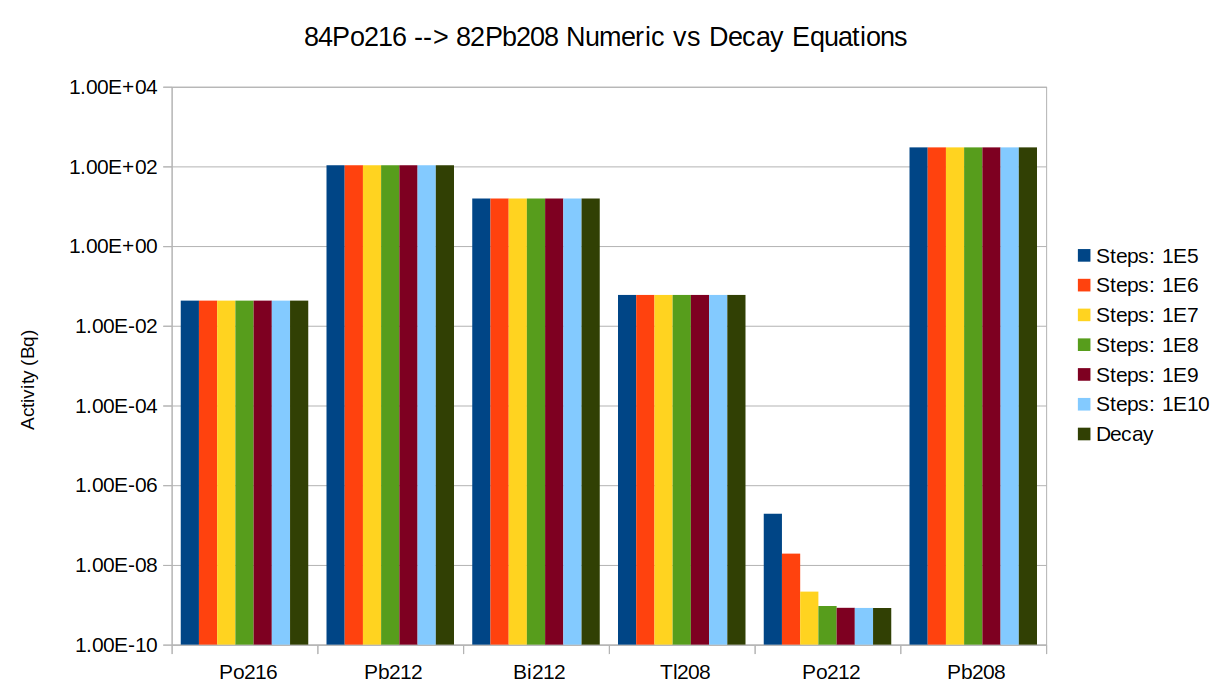
\includegraphics[width=0.7\linewidth]{chapters/activity_code/84po216/decay_84Po216.png}
    \caption{Decay path of Polonium-216}
    \label{fig:decay_equations_vs_analytic}
  \end{center}
\end{figure}

As seen in figure \ref{fig:decay_equations_vs_analytic}, for all but the shortest half life isotope Po-212, the numeric calculations are in good agreement with the decay equations.  As the number of steps increases, and hence the time step decreases, the numerically computed activity for Po-212 also converges to that calculated with the decay equations.

The modified Bateman equation was also tested with several other decay chains against a numeric solution for each chain.  These were the decay of ${}^{49}_{24}Cr$, ${}^{66}_{28}Ni$, ${}^{125}_{55}Cs$, ${}^{213}_{83}Bi$, ${}^{216}_{84}Po$ and ${}^{218}_{86}Rn$.  Apart from a break down in the numeric code, where the half life was comparable to or smaller than the time step, the results from both the equations and the numeric solver were in good agreement.  The full results to this testing are included in appendix \ref{section:decaypo216numeric}.




\subsection{Talys Generated Proton Cross Section Database}
\label{section:activitytalysdb}

Due to a variation in range of energies in the existing cross section data files, the cross section data was computed from scratch using the TALYS code and the BlueBEAR HPC.

A set of proton reaction cross section data files already exist and are updated every few years.  The type and range of data changes between versions of the file.  For example, the \acrshort{tendl}-2014 version contains only elastic and (z,anything) files for (p,Fe56).  The \acrshort{tendl}-2009 file contains a wider ranger of reactions and under 50 data points span the energy range from 0MeV to 200MeV.  The 2019 version contains even more reactions but spans a much shorter energy range, 0MeV to 28MeV, with cross sections given at just under 60 energy points.

The cyclotron used in the experimental work has an energy range up to 40MeV for protons and 53MeV for ${}^{4}He^{2+}$ ions.  To cover this entire range, the TALYS code was used to compute cross section reaction data from 0.01MeV to 62.0MeV in increments of 10KeV, breaking the energy range up into 6,200 data points for each reaction.

\begin{figure}[htb]
\centering
\begin{subfigure}{0.49\textwidth}
  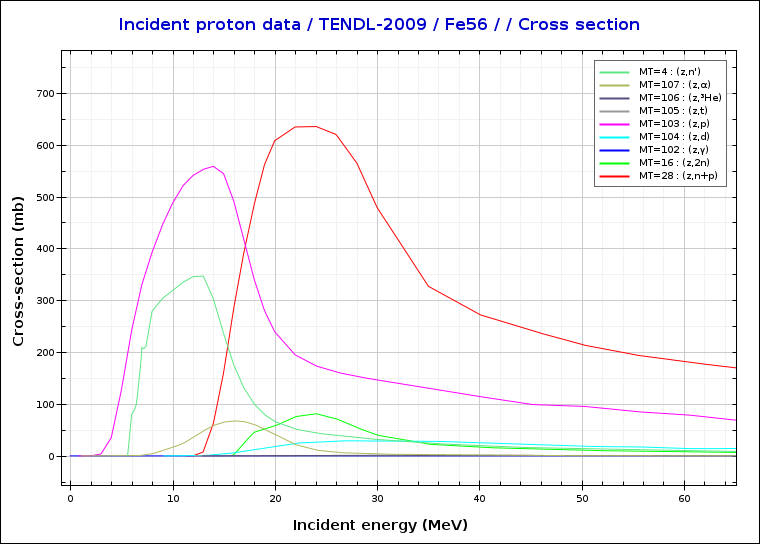
\includegraphics[width=\linewidth]{chapters/activity_code/tendl-fe56/tendl_2009_p_fe56.png}
  \caption{TENDL-2009 cross sections}
  \label{fig:xsdata-tendl2009}
\end{subfigure}\hfil % <-- added
\begin{subfigure}{0.49\textwidth}
  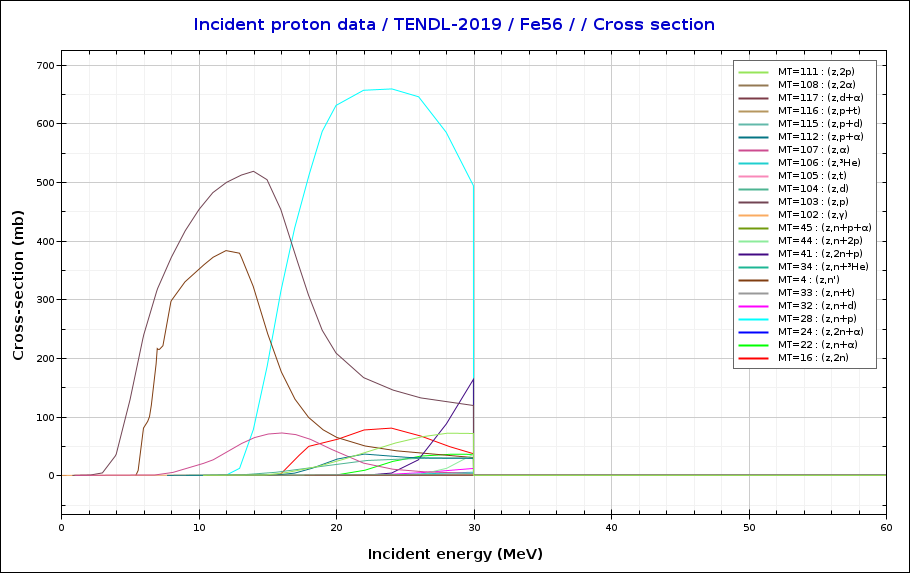
\includegraphics[width=\linewidth]{chapters/activity_code/tendl-fe56/tendl_2019_p_fe56.png}
  \caption{TENDL-2019 cross sections}
  \label{fig:xsdata-tendl2019}
\end{subfigure}

\begin{subfigure}{0.49\textwidth}
  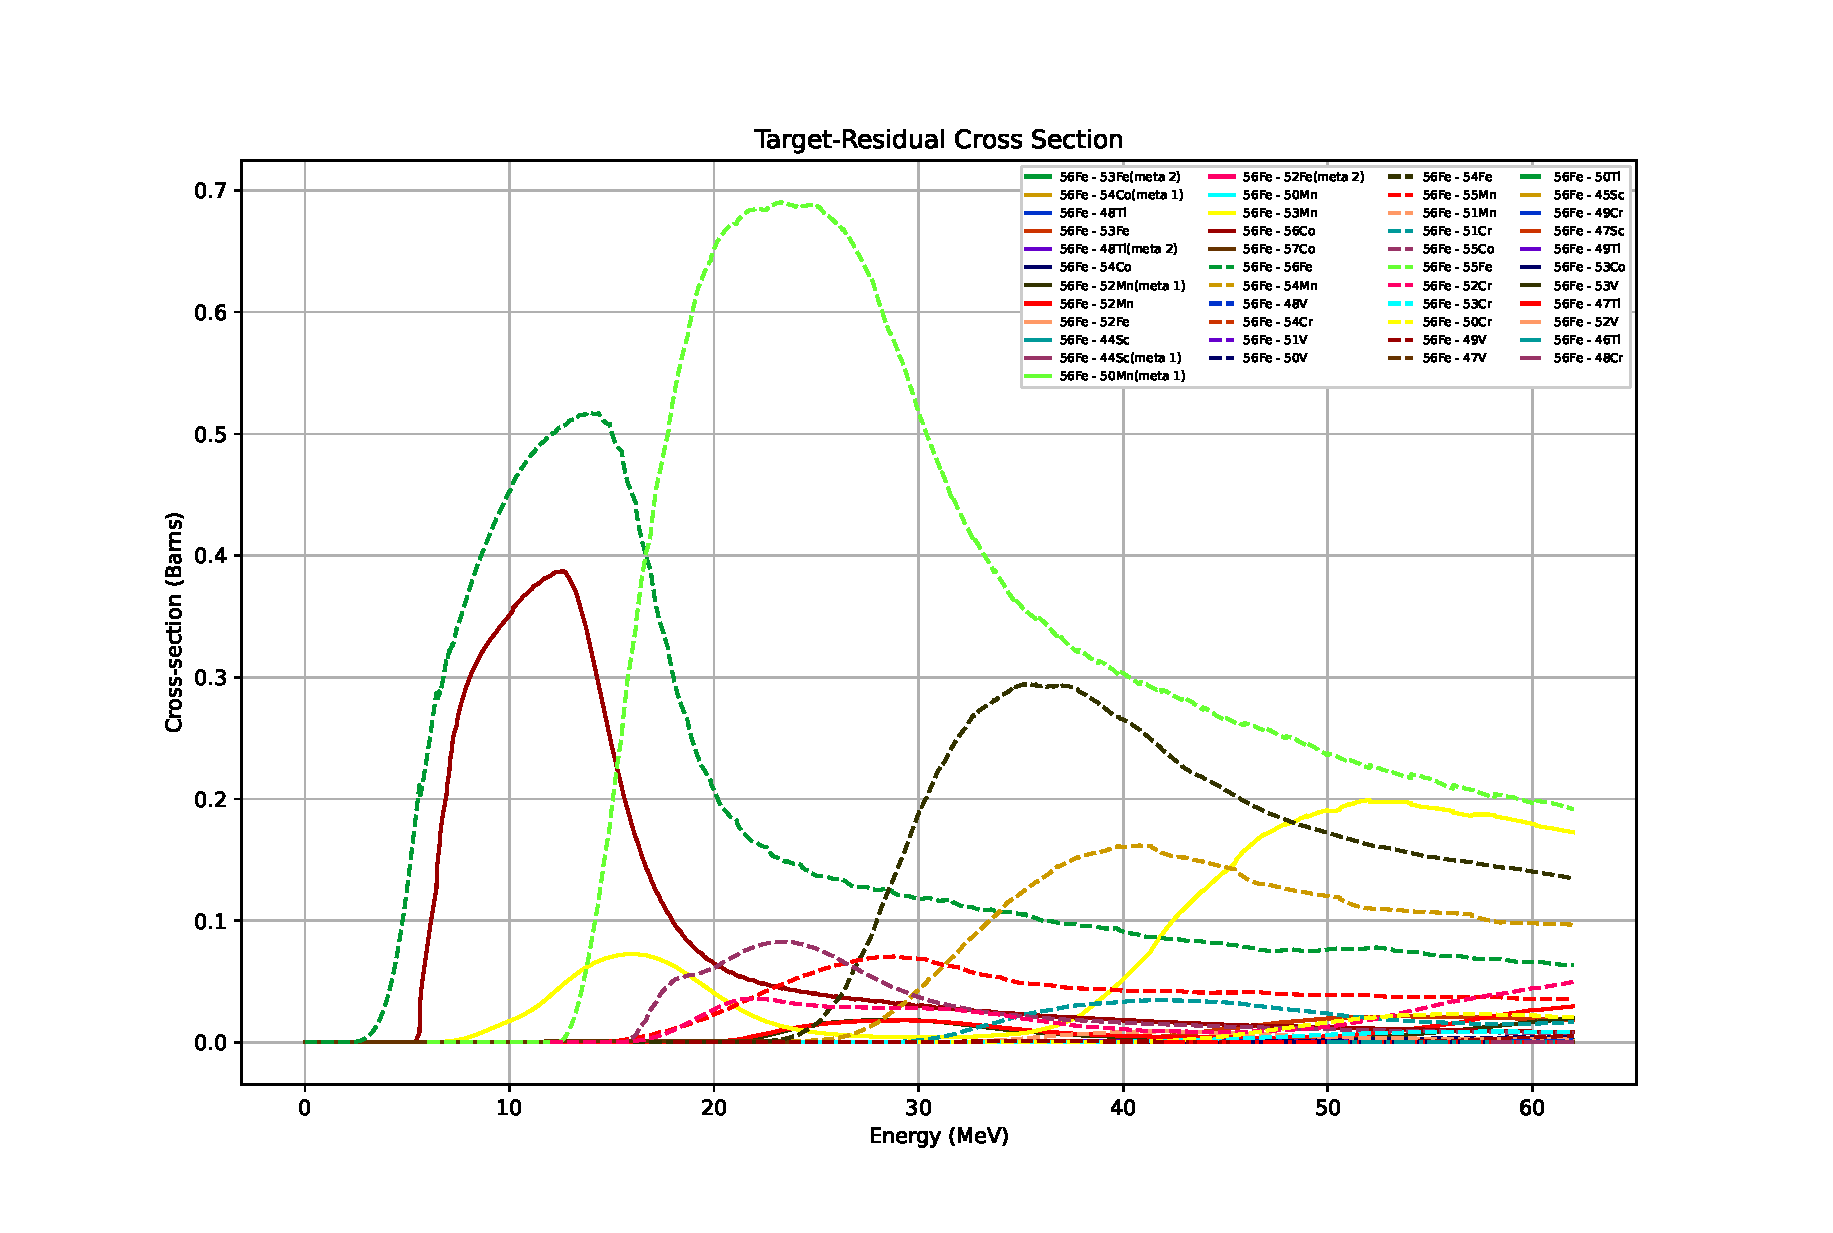
\includegraphics[width=\linewidth]{chapters/activity_code/tendl-fe56/rxs_p_26056_all.eps}
  \caption{TALYS generated residual cross sections}
  \label{fig:xsdata-residual}
\end{subfigure}\hfil % <-- added
\begin{subfigure}{0.49\textwidth}
  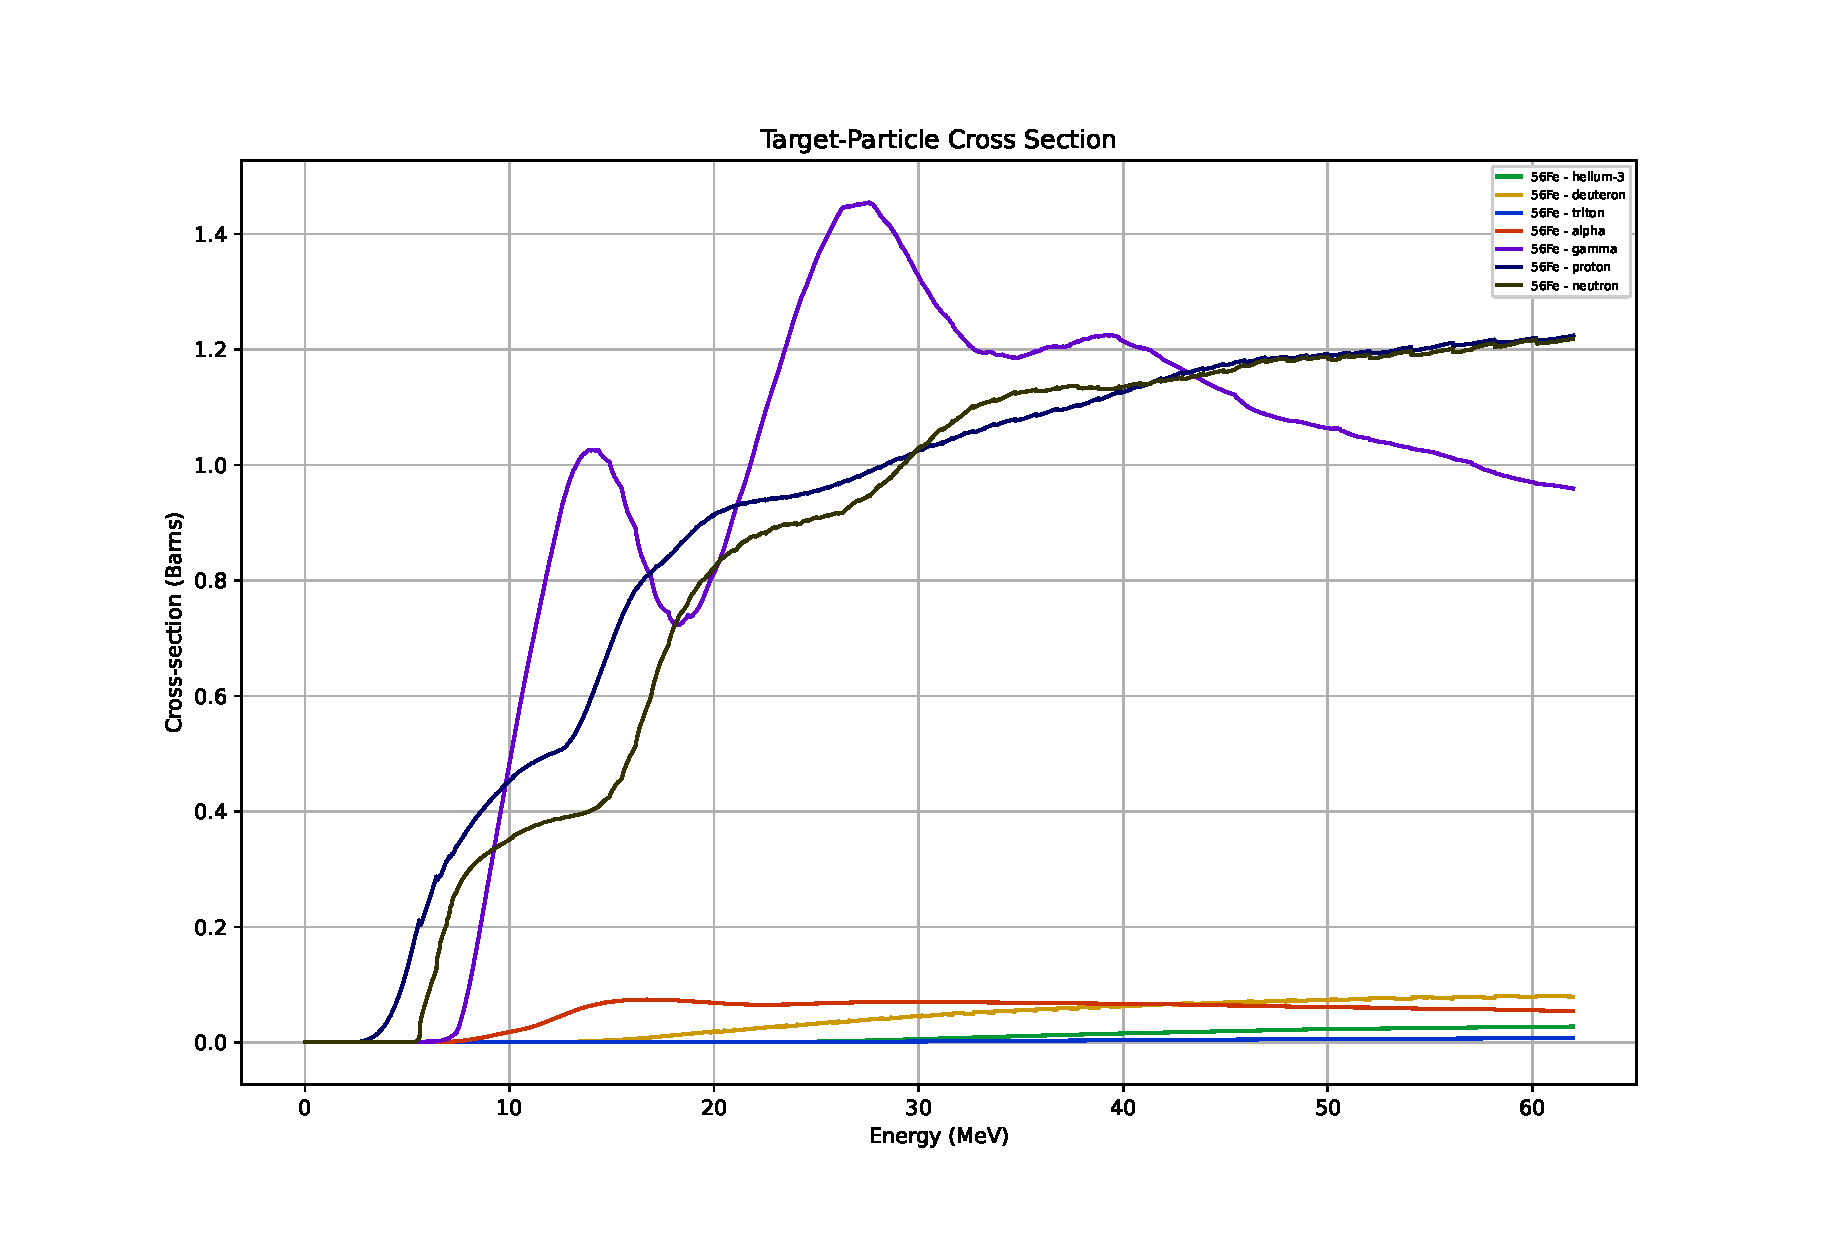
\includegraphics[width=\linewidth]{chapters/activity_code/tendl-fe56/pxs_p_26056_all.eps}
  \caption{TALYS generated particle cross sections}
  \label{fig:activity-v2-residual-6}
\end{subfigure}
\caption{Cross sections for $({}^{56}_{26}Fe, p)$ reactions}
\label{fig:xsdata-particle}
\end{figure}


Limitations of the TALYS code caused the calculations to be processed in batches of either 400 or 600 points.  The data was collated and processed resulting in a datafile of particle production reactions and residual production reactions.  This is accessible through a stand-alone python class that is also a part of the Activity V2 code.

The residual reactions are grouped by target isotope and then by residual isotope, whereas the particle cross sections are grouped by target isotope then particle type.  The computed values are plotted for all available reactions and all residuals for ${}^{56}_{26}Fe$ reactions with protons (figure \ref{fig:xsdata-particle}) and these show a good agreement, although there is a more detailed set of residual isotopes for the generated cross sections.

\begin{lstlisting}[style=sOutputFile,caption={Status report from TALYS database code},label={listing:talysstatus}]
##############################################
    TALYS Cross Section Python Dictionary     
##############################################

               DB STATUS                      

Talys dir:        ../../data/talys
Isotopes file:    ../../data/isotopes.pz
Database load time: 24.489s

Projectiles:    n d p 

Total data points:  18777965

End time:  24.674s
\end{lstlisting}

The complete set of data files, and Python class used to read them, are available to download at:

https://github.com/BenPalmer1983/talys\_xs\_db 

The cross section data output by TALYS was grouped into four main files: elastic\_xs.pz, nonelastic\_xs.pz, particle\_xs.pz and residual\_xs.pz.  All data files that make up this database currently total over 400MB and contain over 18 million data points (listing \ref{listing:talysstatus}), although this could increase if more projectiles and a wide range of energies are added.





\FloatBarrier
\subsection{Ion Trajectory Data}

The \acrshort{srim} code is used to generate ion trajectory data.  This uses a quantum mechanical treatment of ion-atom collisions and statistical algorithms to speed up the process\cite{srimwebsite}.

\begin{figure}[htp]
  \begin{center}
    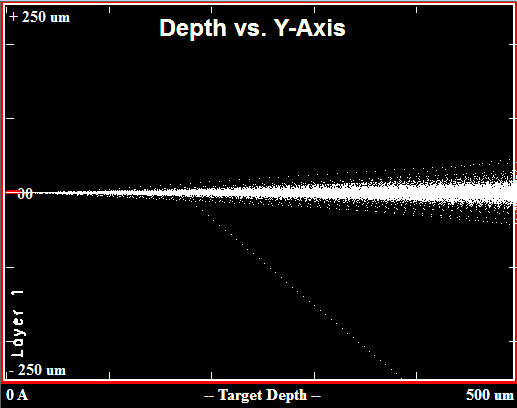
\includegraphics[scale=0.55]{chapters/activity_code/images/ion_transport.png}
    \caption{36MeV Ion Track}
    \label{graph:graph1}
  \end{center}
\end{figure}

The trajectory data files used by both versions of the Activity code will be created using \acrshort{srim} for the required beam energy and target combinations.

\begin{figure}[htp]
  \begin{center}
    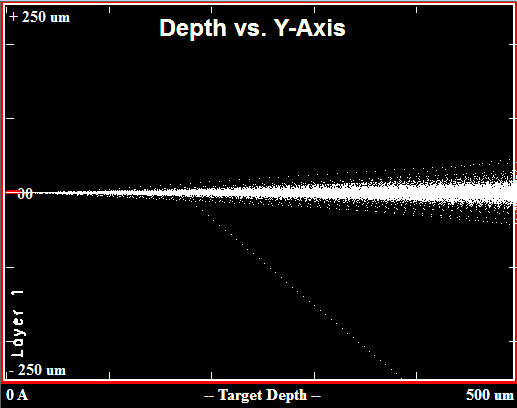
\includegraphics[scale=0.55]{chapters/activity_code/images/ion_transport.png}
    \caption{36MeV Ion Track}
    \label{graph:graph1}
  \end{center}
\end{figure}

The target is set as pure Iron, and due to the way \acrshort{srim} functions, the structure type is inconsequential.  At just 0.5mm in thickness, the 36MeV ions pass through the targets and exit with an energy above 30MeV, and the exyz.txt data file covers this range of ion energies.


\subsection{Activity Code Assumptions}

A number of assumptions have been made for both codes to simplify the model.  These may be addressed in future versions if development of the code continues.  The flux of the beam is assumed to be constant at any depth into the material.  Charged particle irradiation is ignored completely from the decay of radioactive isotopes in the target, and the amount of beta radiation may determine how the target is handled.

Gammas are assumed to be emitted isotropically and degrade only due to the increase in surface area as the distance from the source increases.  No consideration is given to the dispersion of radioactive isotopes through the target material, how much material the gammas must pass through or how much air they must go through in order to reach the person (or measuring device).

These assumptions and possible improvements are considered in chapter \ref{chapter:futurework}.


\FloatBarrier



\subsection{Foil Activation by Neutron Irradiation}

An additional feature was added to the Activity V2 code to estimate neutron activity based on the existing code developed to calculated ion activation.  It is a simple non-transport neutron activation code, used to estimate the activity and subsequent cooling of materials irradiated by neutrons.  A single energy neutron flux or Maxwell-Boltzmann distribution may be selected by the user and the TALYS generated database is used to provide cross sections for calculating reaction rates.  Finally, the previously derived extended Bateman equations are used to calculate isotopes at time t after irradiation begins.


\FloatBarrier
\section[Simulating with SRIM - Iron]{Simulating Proton Irradiated Iron with SRIM}

The trajectory data used by the activity code(s), and also to estimate the ${}^{55}_{27} Co$ activity, was provided by SRIM.  An input configuration was set with Iron as the target material and protons as the projectile ion.  The sample depth was set to at least the target thickness, 0.5mm.  The activity code truncates the data to fit the target thickness, so a much larger depth, say 1m, could be set in SRIM to ensure all the ions stop within the simulated target, and this data file may be reused for targets of varying thicknesses.

\begin{figure}[htb]
\centering
\begin{subfigure}{0.49\textwidth}
  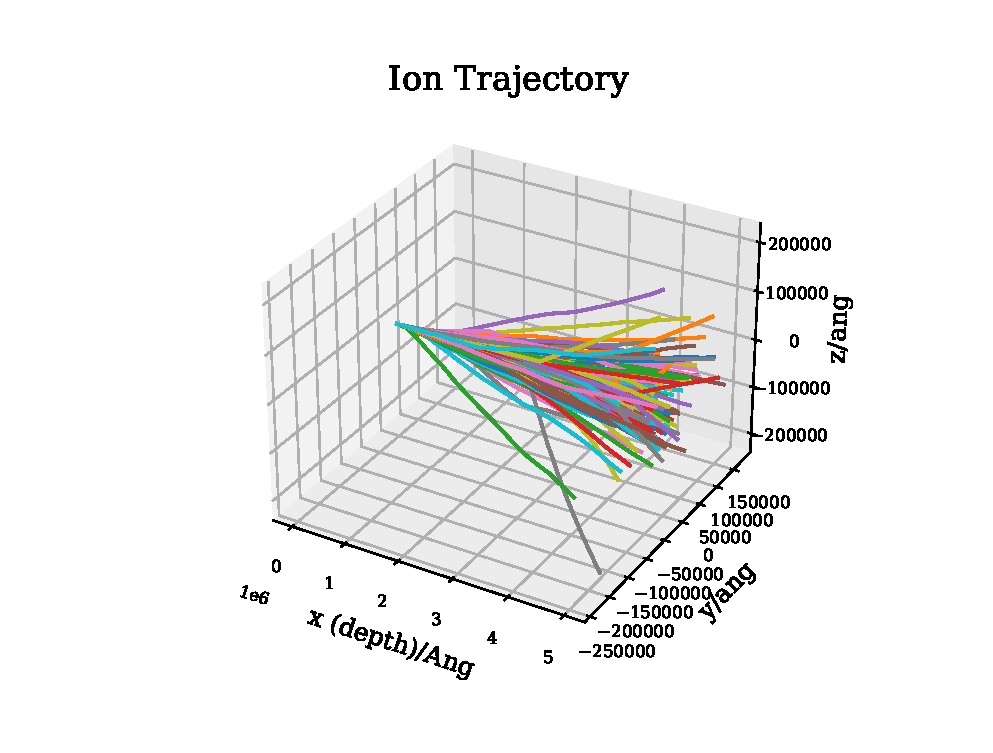
\includegraphics[width=\linewidth]{chapters/activity_code/images/trajectory_3d_500um.eps}
  \caption{Proton trajectory}
  \label{fig:iontrajectory1}
\end{subfigure}\hfil
\begin{subfigure}{0.49\textwidth}
  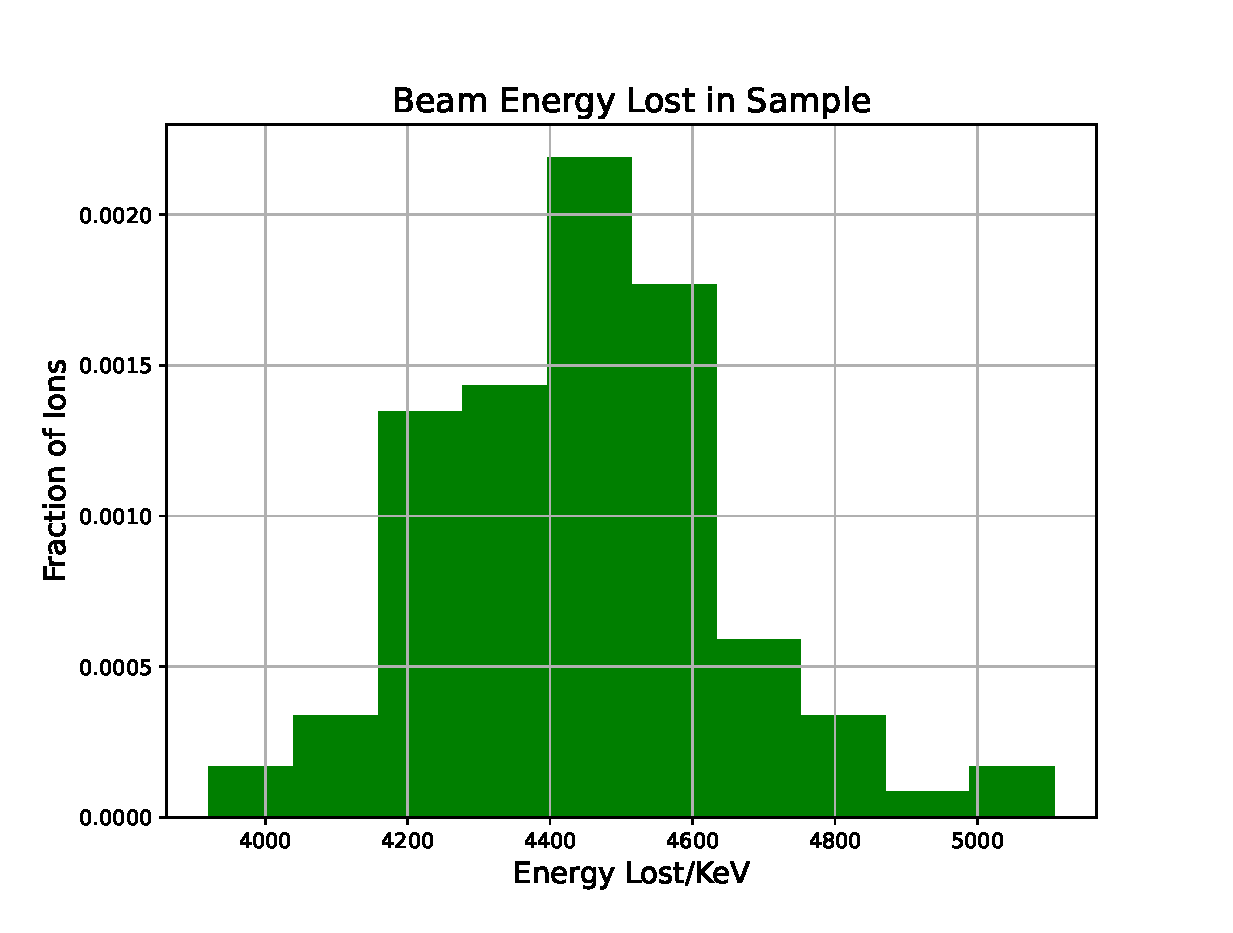
\includegraphics[width=\linewidth]{chapters/activity_code/images/energy_lost_500um.eps}
  \caption{Histogram of energy lost passing through target}
  \label{fig:energylost1}
\end{subfigure}
\begin{subfigure}{0.49\textwidth}
  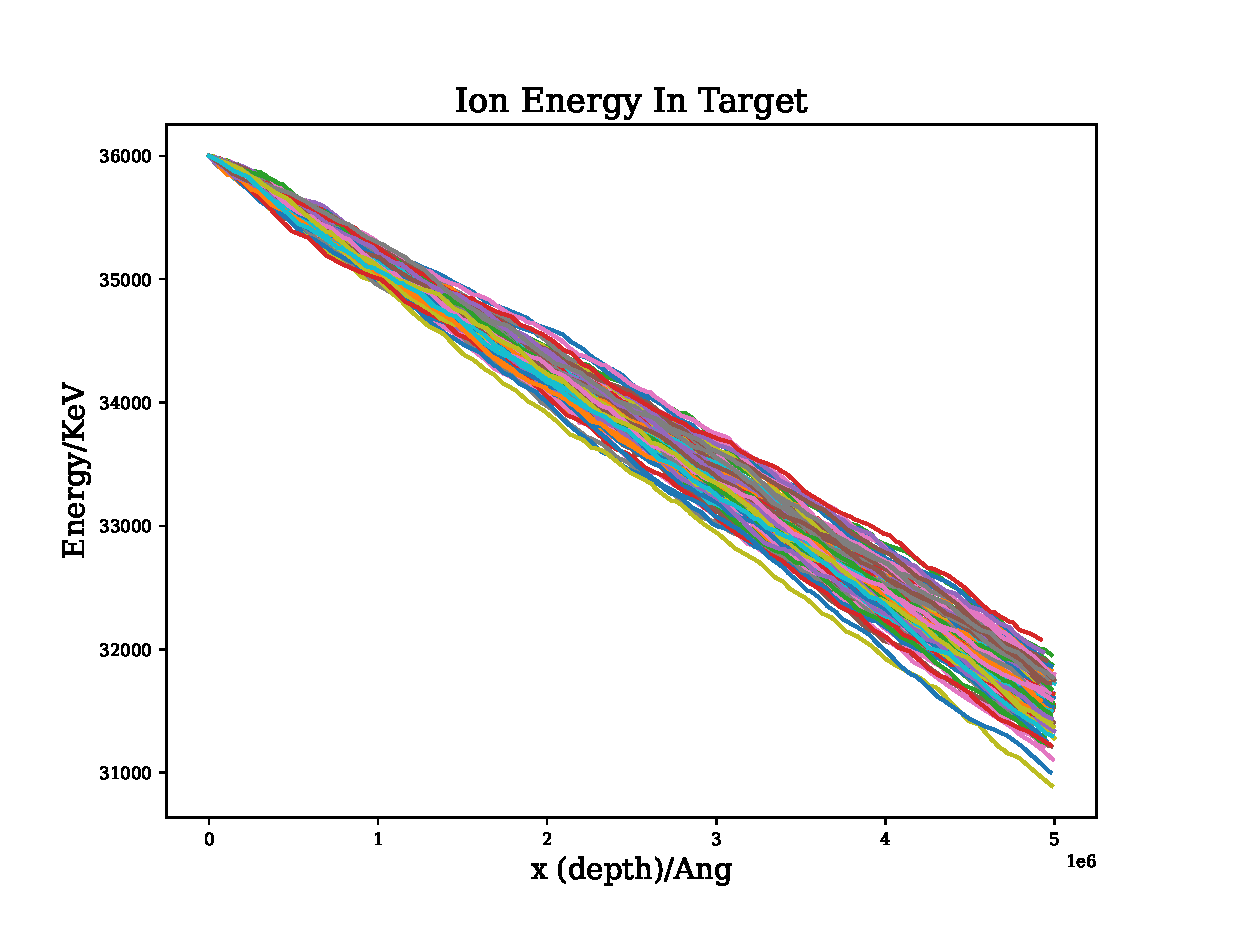
\includegraphics[width=\linewidth]{chapters/activity_code/images/energy_depth_500um.eps}
  \caption{Energy vs target depth}
  \label{fig:fe36mevenergydepth}
\end{subfigure}
\caption{Protons through a 0.5mm thick iron target - 100 proton histories}
\label{fig:xsdata-particle1}
\end{figure}

The ions travelling through the thin 0.5mm target lose between 4MeV and 5MeV (figure \ref{fig:energylost1}) as they pass, and they do so quite smoothly (figure \ref{fig:fe36mevenergydepth}).  The majority of the energy is lost smoothly through electronic stopping.  

The ion trajectory plot shows the deflection of ions in both the y and z axis.  A large percentage of the ions here deviate very little from a straight pass through, but several are deflected by quite a large angle.  Within the activity computer codes, these ions deflected ions will travel a greater distance through the target.  The only cutoffs applied to the ion trajectory data are either the ion reaching 0MeV or travelling more than the depth in the x-axis.  Any ions travelling a large distance in the y or z axis are still determined to be within the target.

\begin{figure}[htb]
\centering
\begin{subfigure}{0.49\textwidth}
  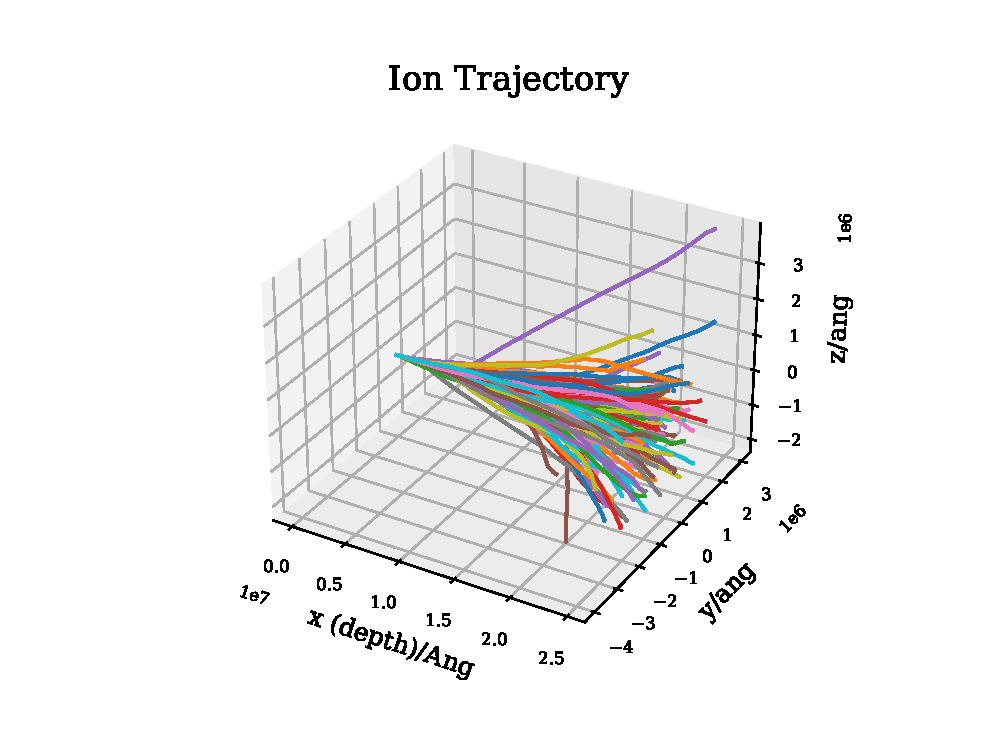
\includegraphics[width=\linewidth]{chapters/activity_code/images/trajectory_3d_full.eps}
  \caption{Proton trajectory}
  \label{fig:iontrajectory2}
\end{subfigure}\hfil
\begin{subfigure}{0.49\textwidth}
  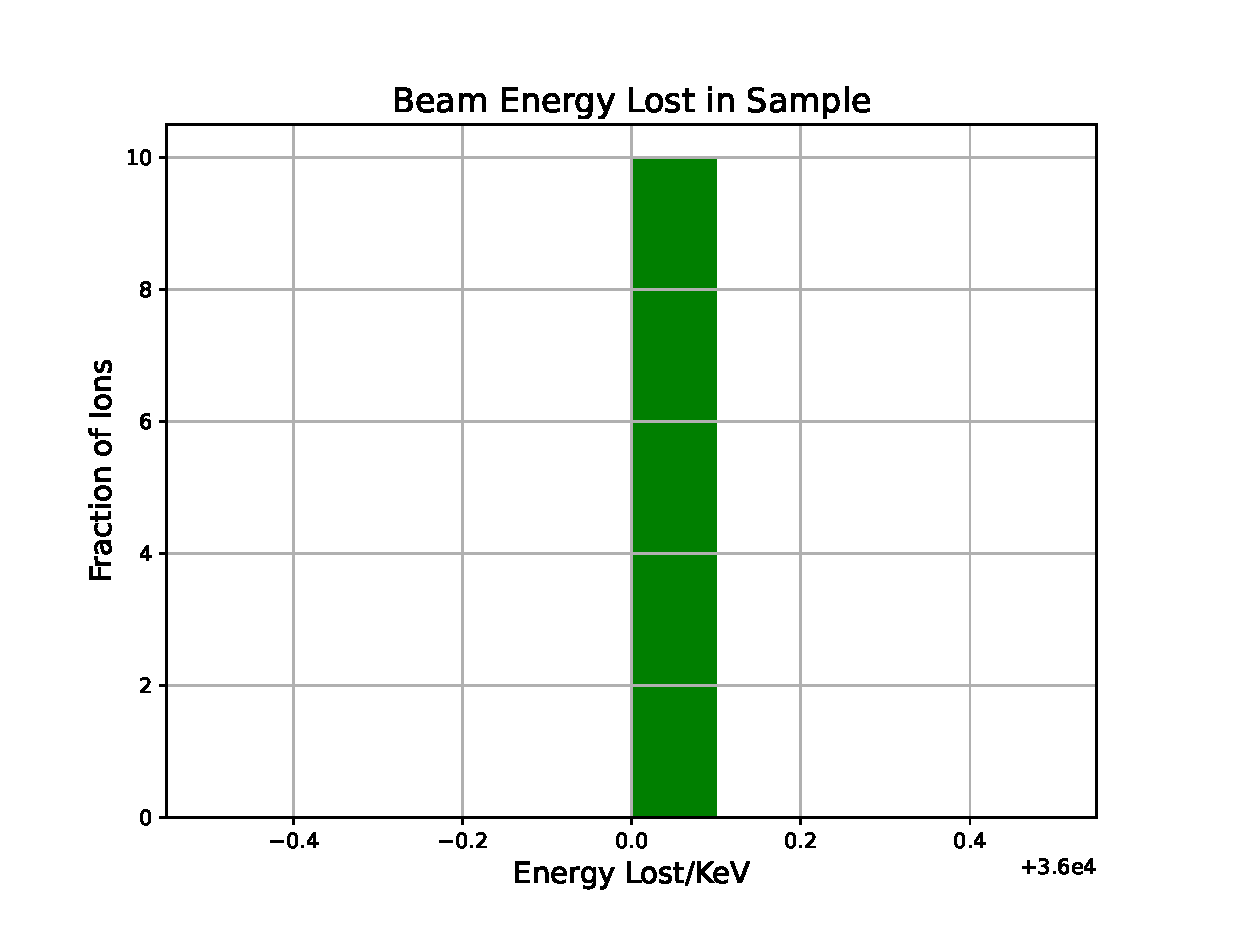
\includegraphics[width=\linewidth]{chapters/activity_code/images/energy_lost_full.eps}
  \caption{Histogram of energy lost passing through target}
  \label{fig:energylost2}
\end{subfigure}
\begin{subfigure}{0.49\textwidth}
  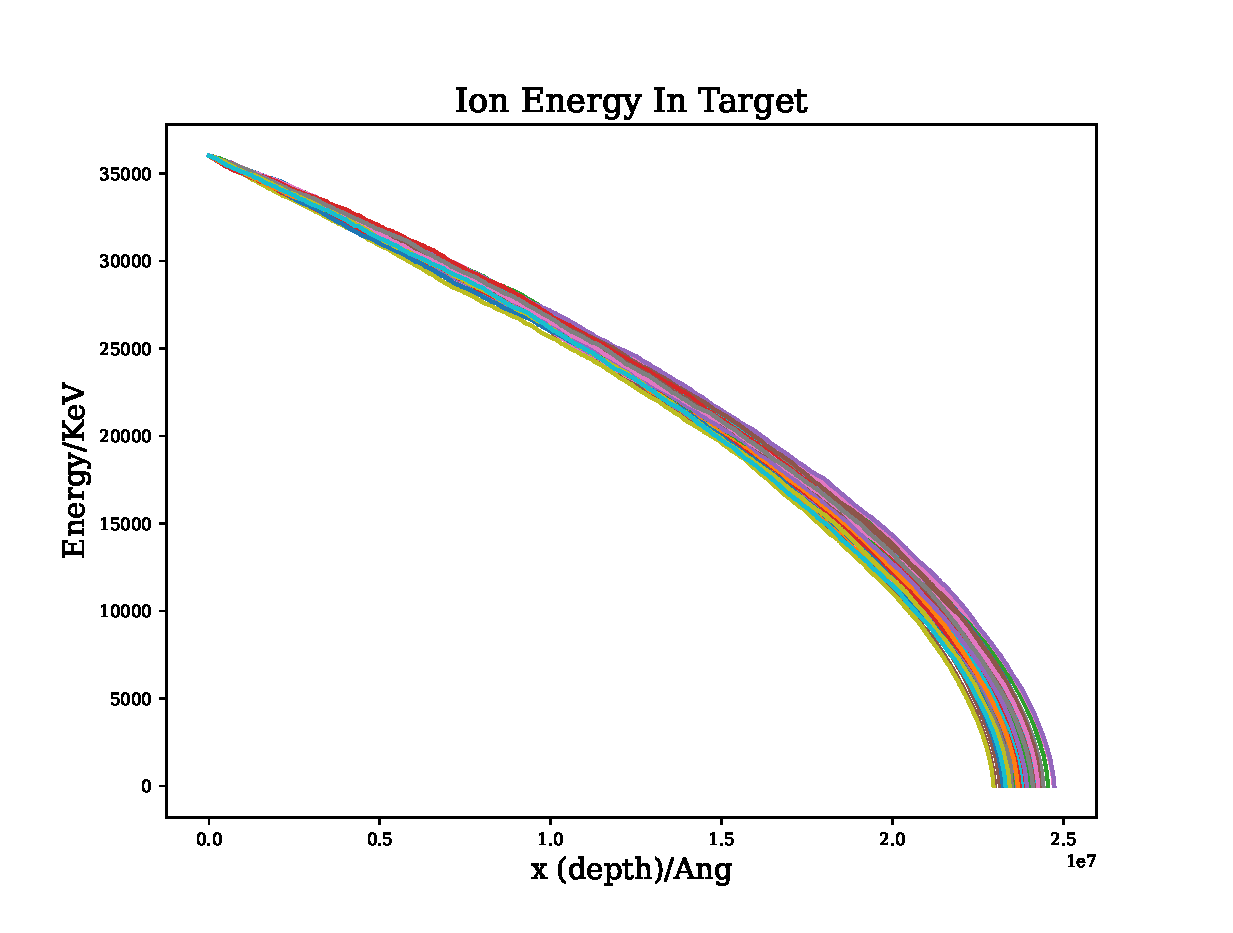
\includegraphics[width=\linewidth]{chapters/activity_code/images/energy_depth_full.eps}
  \caption{Energy vs target depth}
  \label{fig:fe36mevenergydepthfull}
\end{subfigure}
\caption{Protons through target thick enough to stop all ions - 100 proton histories}
\label{fig:xsdata-particle2}
\end{figure}

As the thickness of the iron is increased, all the energy is lost to the iron target, and this loss of energy occurs within a shorter range in the remaining quarter of a millimetre depth of the iron target (figure \ref{fig:iontrajectory2}).










\section{Cyclotron Irradiated Iron}

\subsection{Cyclotron Beam Line}

The Scanditronix MC40 cyclotron at the University of Birmingham has several beamlines and is capable of accelerating protons, deuterons, Helium 3 and Helium 4 with fluxes and energy ranges detailed in table \ref{table:scanditronixlimits}.  After running a simulation with \acrshort{srim}, the 36MeV protons were expected to create an average of 15.8 vacancies each.

\begin{table}[h]
\begin{center}
\begin{tabular}{c c c c}
\hline\hline
Particle & Energy (MeV) & Max Current (micro A) & Flux (ions per second)\\
\hline\hline
p & 8-40 & 60 & $3.75 \times 10^14$ \\
d & 8-40 & 30 & $1.87 \times 10^14$ \\
${}^4 He^{2+}$ & 8-53 & 30 & $9.36 \times 10^13$ \\
${}^3 He^{2+}$ & 4-20 & 60 & $1.87 \times 10^14$ \\
\hline\hline
\end{tabular}
\end{center}
\caption{Beam Characteristics of the Scanditronix MC-40}
\label{table:scanditronixlimits}
\end{table}

The cyclotron is located in one room, and several beam lines run from the cyclotron to other rooms in the cyclotron building.  The operation room is separate from the cyclotron and beam line rooms (figure \ref{fig:cyclotronlayout}).

\begin{figure}[htp]
	\minipage{0.49\textwidth}
  \begin{center}
    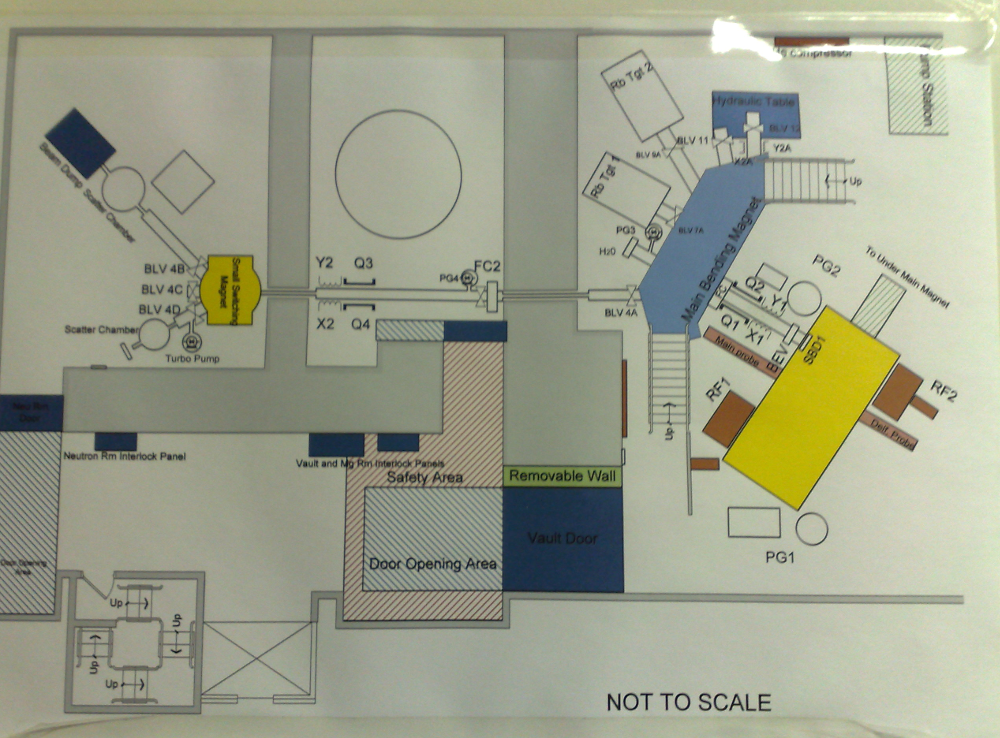
\includegraphics[width=\linewidth]{chapters/activity_code/images/cyclotron_layout.png}
    \caption{Cyclotron layout - main hall and beam lines}
    \label{fig:cyclotronlayout}
  \end{center}
	\endminipage\hfill
	\minipage{0.49\textwidth}
  \begin{center}
    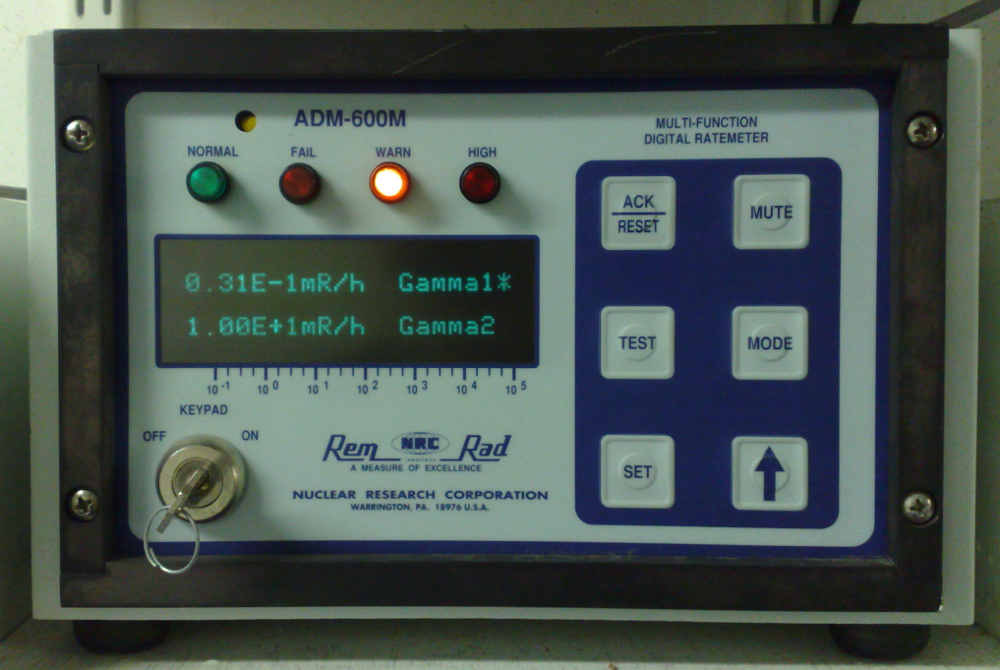
\includegraphics[width=\linewidth]{chapters/activity_code/images/gamma_warning.png}
    \caption{Gamma warning alarm during 0.5 microamp 36MeV proton irradiation of iron }
    \label{fig:gammawarning}
  \end{center}
	\endminipage\hfill  
\end{figure}

The iron sample was held perpendicular to the beam line, with the ions passing through the 0.5mm thickness of the sheet.  The beam area was approximately $6.4 \times 10^{-5} m^2$, irradiating a volume of approximately $3.2 \times 10^{-8} m^3$.  The target was irradiated for 300 seconds at 0.5 micro amps and it was expected to cause over $1.4 \times 10^{16}$ displacements within the volume of iron targetted by the beam.  With a number density of approximately $8\times10^{28}$ atoms per cubic meter, giving a relatively low damage dose, when compared to that expected over the lifetime of a component within the reactor, of $5 \time 10^{-6}$ \acrshort{dpa}.

During irradiation, the amount of gamma radiation released was enough to trip the alarm for the room (figure \ref{fig:gammawarning}).  The proton fluence was less than 1\% of the maximum fluence capable of being produced by the cyclotron, so this was definitely a concern.  To increase the damage dose, and keep to a shorter period of time, the current would most probably be increased to a much higher percentage, also increasing the rate of Gammas produced during irradiation.

Preliminary investigations with SRIM into the stopping distance of protons in a range of materials shows 36MeV ions stop within 3mm in Iron and Steel(figure \ref{fig:stoppingdistanceprotons}).

\FloatBarrier
\begin{figure}[h]
  \begin{center}
    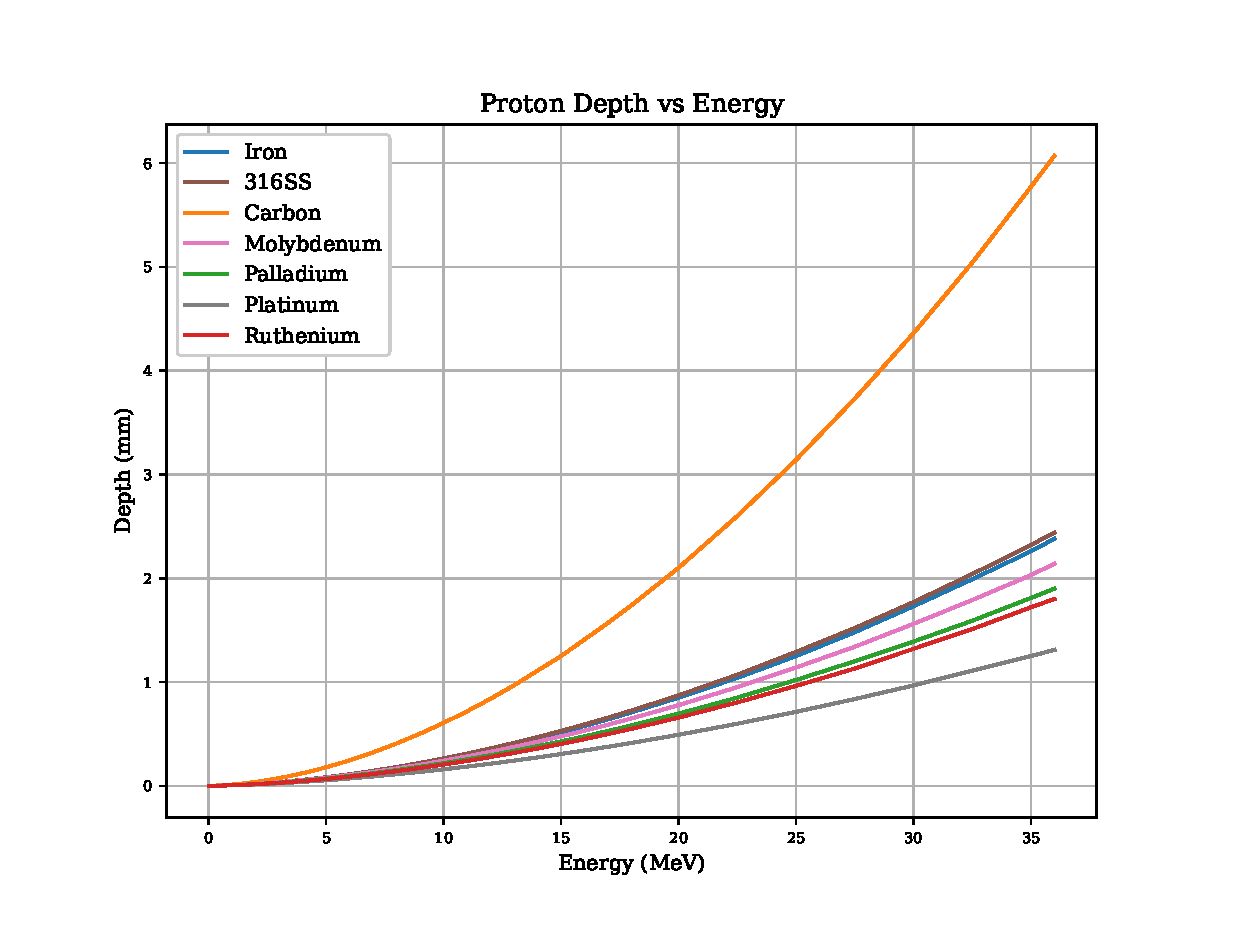
\includegraphics[width=0.7\linewidth]{chapters/activity_code/proton_stopping.eps}
    \caption{Proton stopping distances in various materials}
    \label{fig:stoppingdistanceprotons}
  \end{center}
\end{figure}

It is clear that 3mm thick samples of Iron or Steel will completely stop 36MeV protons and 1mm of the same is enough to stop any with an energy of 20MeV or less.


\subsection{Creation of Cobalt-55}

${}^{55}_{27} Co$ is a relatively short lived isotope with a half life of 17.5 hours and this is a concern to health during and shortly after irradiation.  Isotopes with a long half life are not as active in small quantities, and those with very short half life decay away quickly.  ${}^{55}_{27} Co$ decays into another radioactive isotope, ${}^{55}_{26} Fe$, which then decays into ${}^{55}_{25} Mn$ (figure \ref{fig:DecayPathCo55}).  The second step in the decay chain is 2.73 years, so the first step with a much shorter half life will be responsible for the majority of the radiation shortly after being irradiated by protons.

\FloatBarrier
\begin{figure}[h]
  \begin{center}
    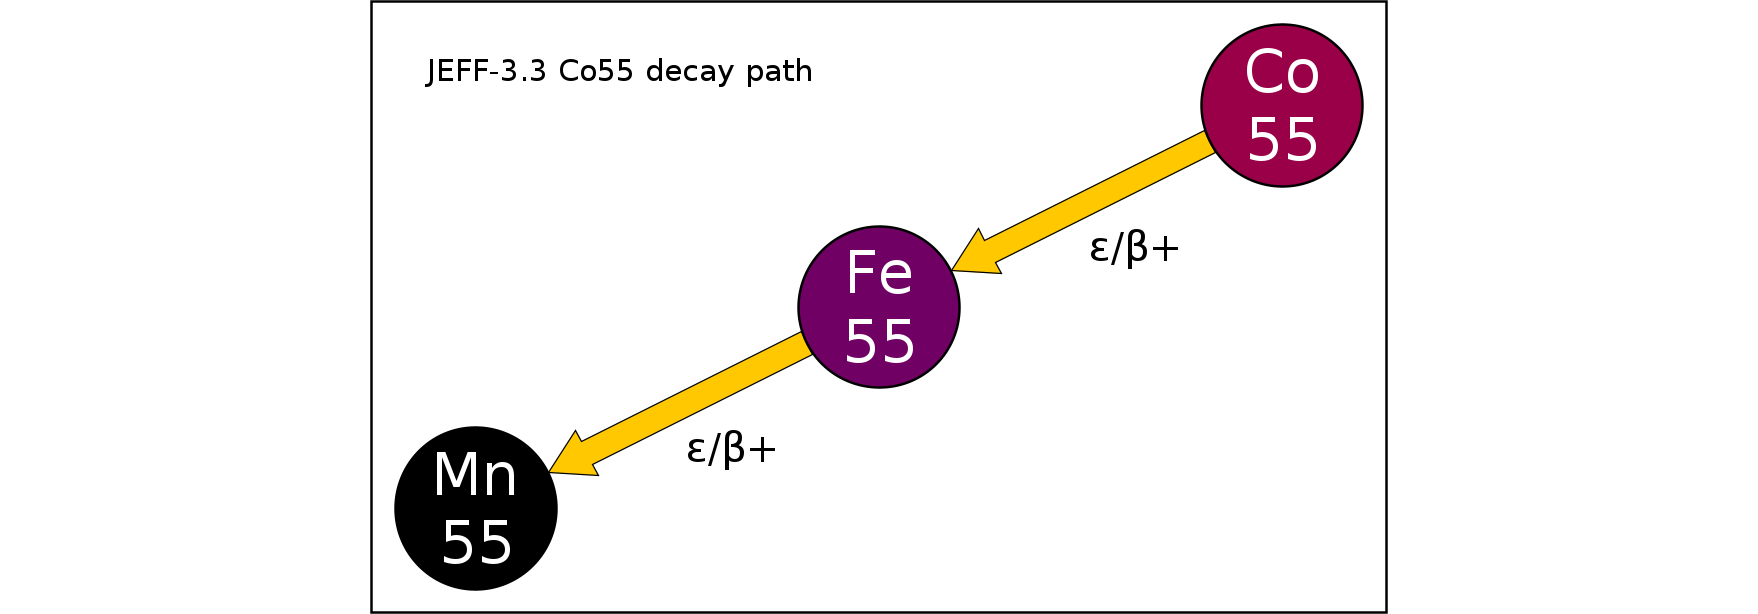
\includegraphics[width=0.5\linewidth]{chapters/activity_code/fe-co55/Co55_decay_path.png}
    \caption{Decay path of Cobalt-55}
    \label{fig:DecayPathCo55}
  \end{center}
\end{figure}

\FloatBarrier
The decay of ${}^{55}_{27} Co$ will produce a range of gammas (figure \ref{fig:Co55GammaIntensity}), but one in particular to focus on when measuring the radioactivity is the 931KeV gamma with an intensity of 75\%.

\FloatBarrier
\begin{figure}[h]
  \begin{center}
    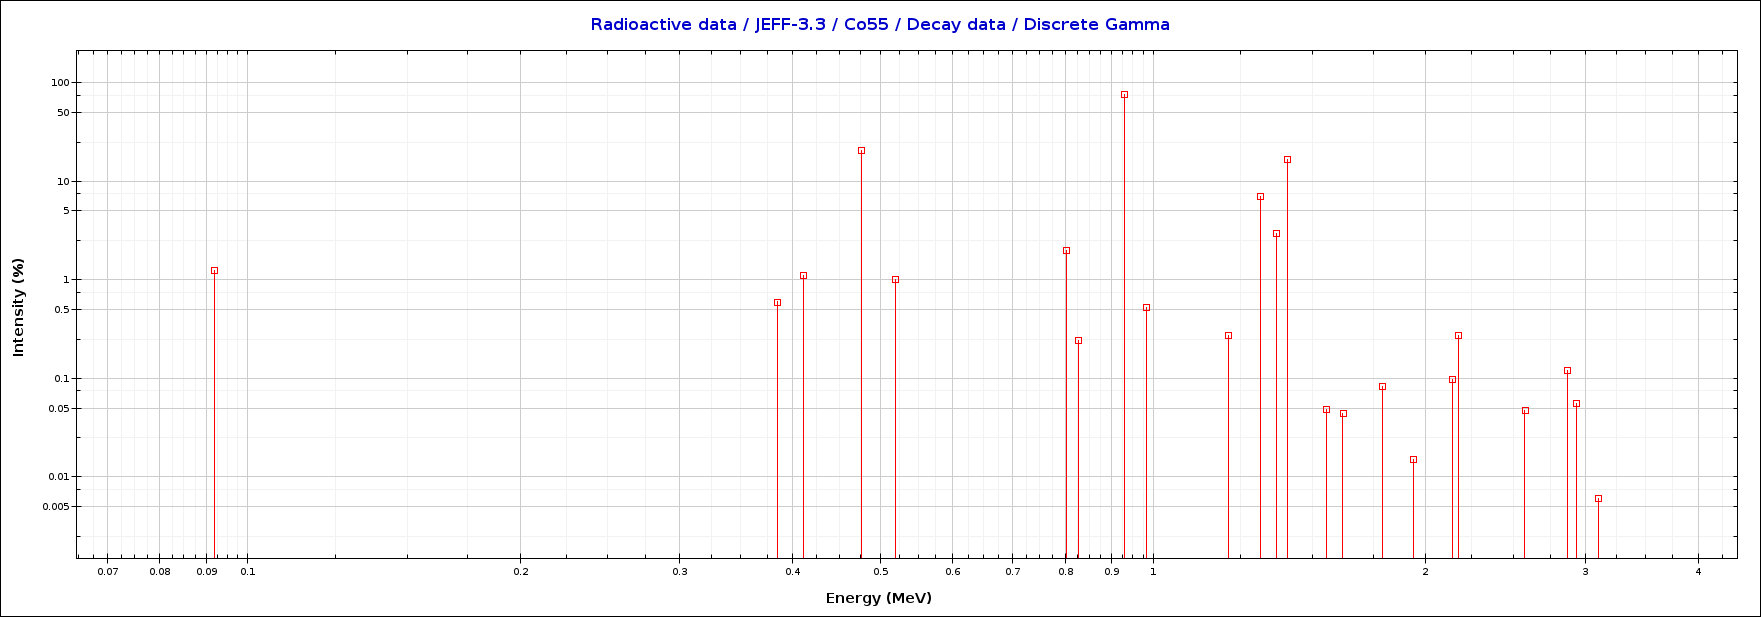
\includegraphics[width=0.9\linewidth]{chapters/activity_code/fe-co55/Co55_discrete_gamma.png}
    \caption{Cobalt-55 Gamma Intensity Plot}
    \label{fig:Co55GammaIntensity}
  \end{center}
\end{figure}

\FloatBarrier

The stable isotope ${}^{54}_{26} Fe$  makes up almost 6\% of natural iron, and one reaction possibility with a proton results in ${}^{55}_{27} Co$ and a gamma, ${}^{54}_{26} Fe (p, \gamma) {}^{55}_{27} Co$.  The most abundant isotope in natural Iron also has a route to transmute to ${}^{55}_{27} Co$ through the capture of a proton and the loss of two neutrons, ${}^{56}_{26} Fe (p, 2n) {}^{55}_{27} Co$.

Due to the short half-life and intensity of the 931KeV gamma, this peak was measured in particular after irradiating the iron target.  It was also estimated manually using the \acrshort{tendl}-2009 and \acrshort{tendl}-2019 cross section databases.




\subsection{Measurement of Sample Activity}

The sample was too radioactive to safely handle immediately after irradiation, so it was left to cool for several days before taking measurements.  After it had cooled, a high purity germanium detector (figure \ref{fig:hpge}) was used to measure the activity of the irradiated sample.  The radioactivity was measured using a high purity germanium detector which was calibrated to detect approximately 4 out of every 100 gammas emitted.  

\begin{figure}[htp]
  \begin{center}
    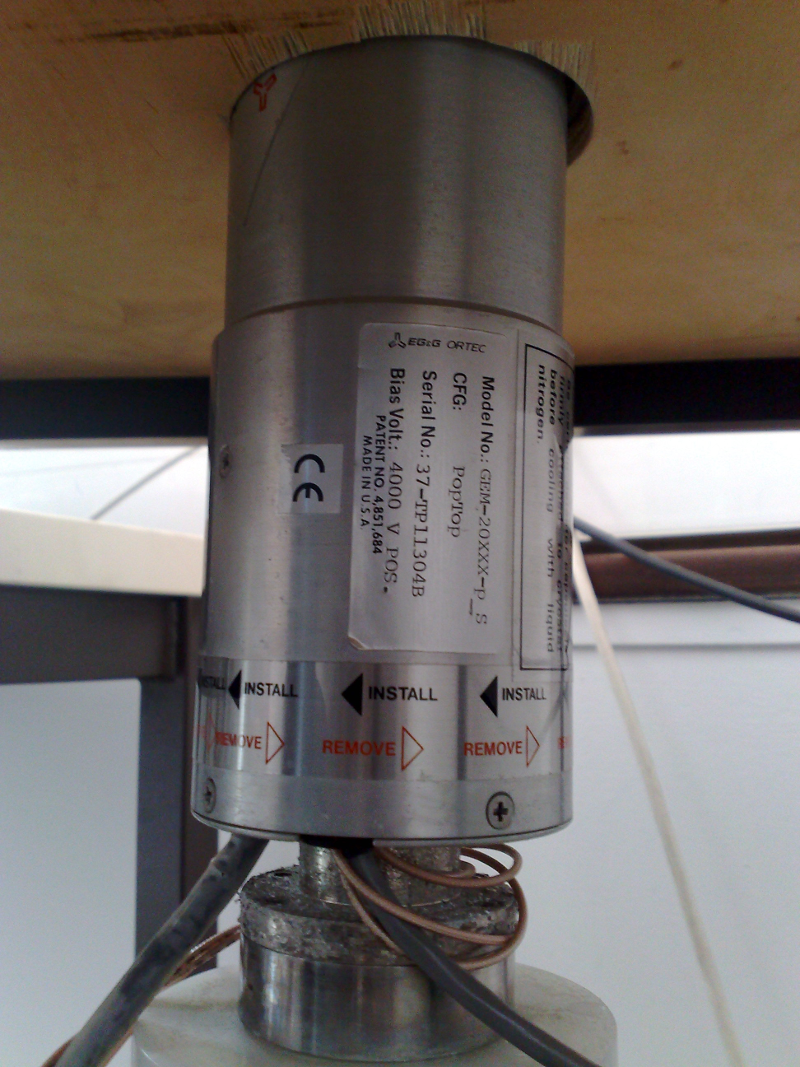
\includegraphics[scale=0.8]{chapters/activity_code/images/hpge.png}
    \caption{High Purity Germanium Detector}
    \label{fig:hpge}
  \end{center}
\end{figure}

The detector and preamplifier are both cooled by liquid nitrogen to 77K, as the band-gap of germanium is 0.7eV and the thermal motion of electrons and nuclei at higher temperatures would induce currents causing noise and interference in the detector.  As a gamma ray enters the detector it creates an electron-hole pair in the medium of the detector.  The holes and electrons are attracted to the center and to the outer cylinder of the detector, or vice versa.




\begin{lstlisting}[style=sMaestro,caption={Maestro 931KeV Peak Measurement},captionpos=b]
RANGE: 617 = 911.51keV to 649 = 958.79keV
AREA : Gross = 2127168 Net = 1342565 +/- 2207
CENTROID: 631.74 = 933.29keV
SHAPE: FWHM = 6.82 FW(1/5)M = 10.06
ID: Bi-214 at 934.05keV
Corrected Rate = 35349.26 +/- 58.11 cA
\end{lstlisting}

The gamma counts were recorded over a range of 0MeV to 3MeV (figure \ref{fig:measuredgammacounts}). Correcting the measured count for the 931KeV peak, to account for the geometry and detector, the count rate for 931KeV gamma rays from ${}^{55}_{27} Co$ was measured at $4.43\times10^4 +/- 1.05 \times 10^3$ counts per second.

\begin{figure}[ht] 
  \centering
  \begin{minipage}[b]{0.85\linewidth}
    \centering
    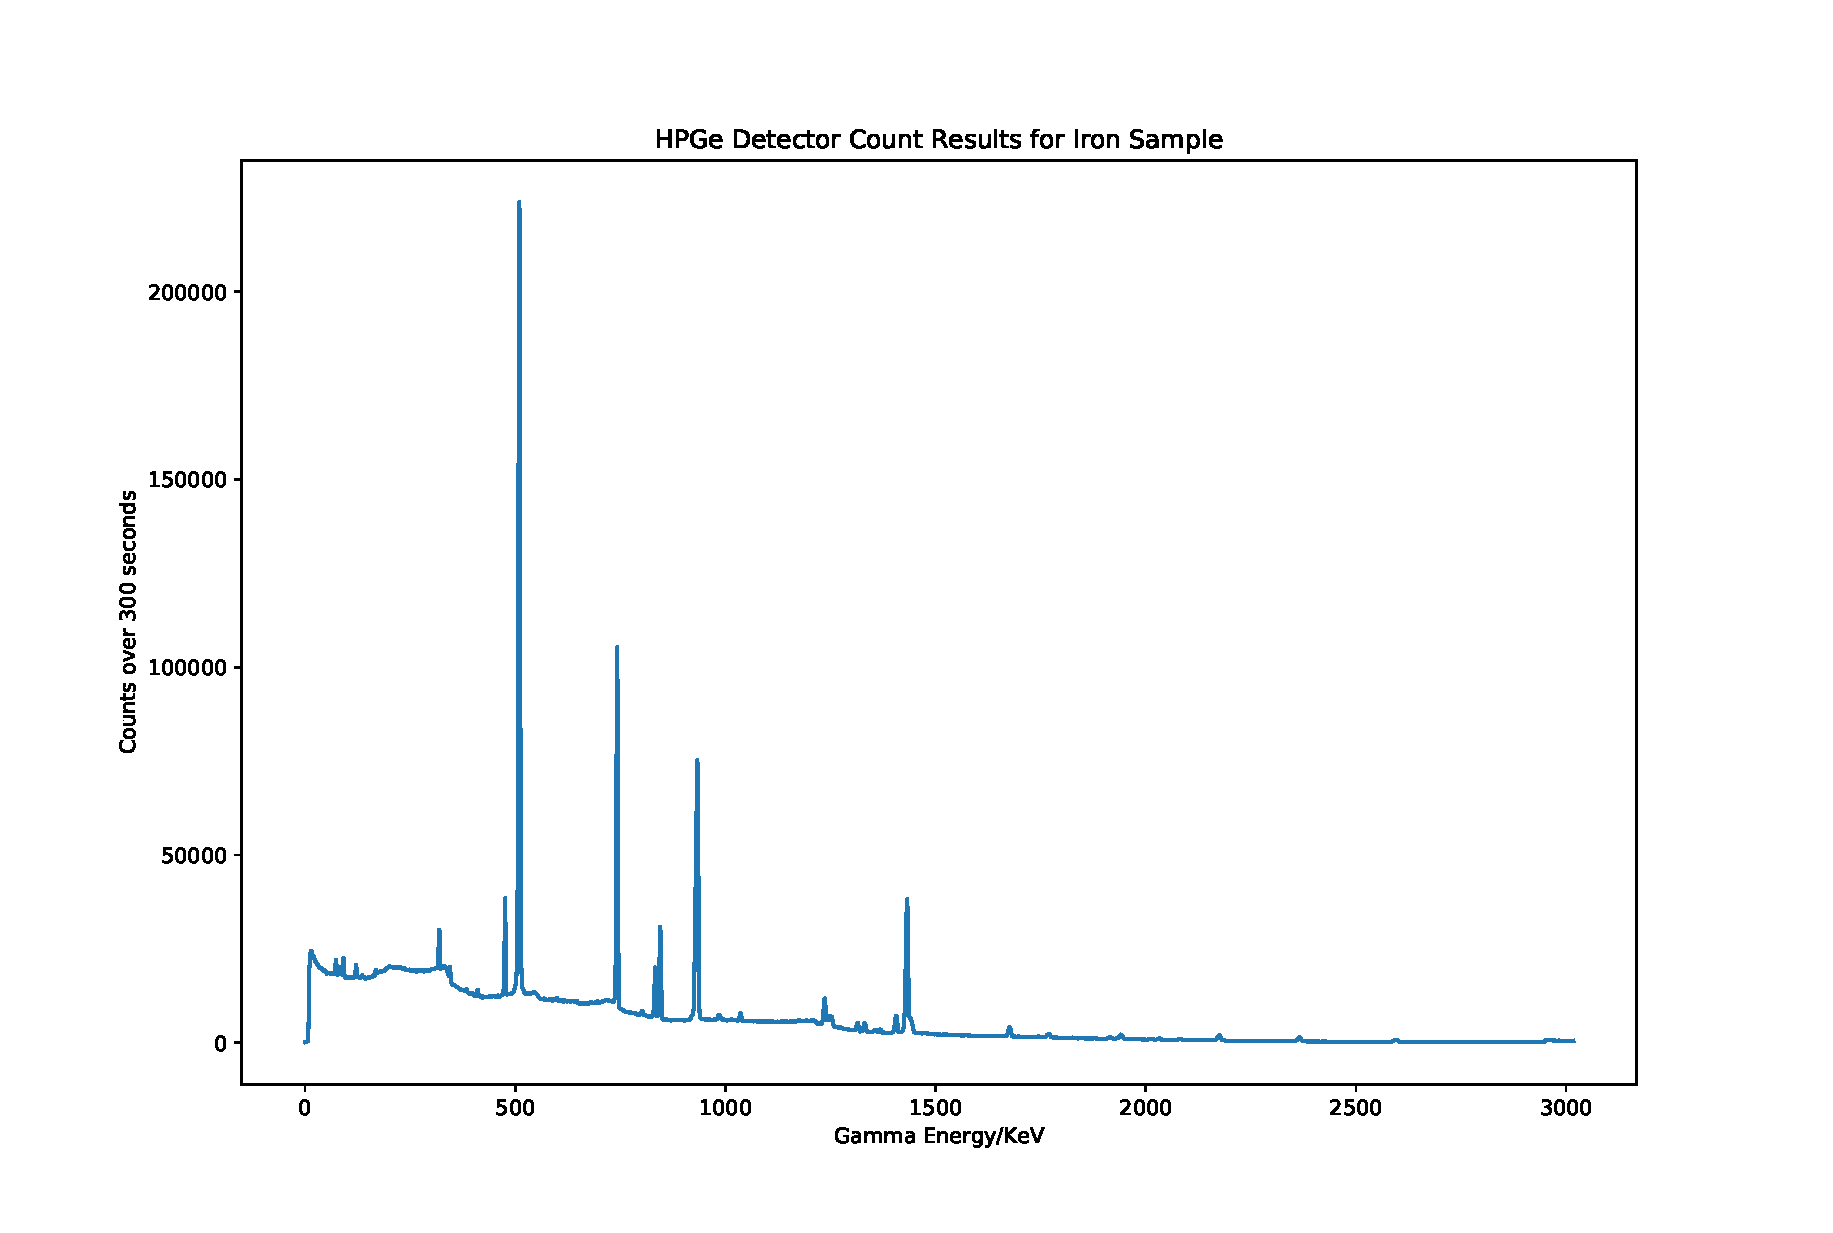
\includegraphics[width=.9\linewidth]{chapters/activity_code/experimental/gamma_counts.eps} 
    \caption{Gamma counts from the irradiated iron target over 300 seconds}  
    \label{fig:measuredgammacounts}
  \end{minipage}%%
\end{figure}

There are several decay modes that contribute to the radioactivity of the sample, and the largest contributors to gamma emission also undergo either electron capture or $\beta +$ emission.  The decay paths are:

\begin{itemize}
\item ${}^{55}_{27}Co \xrightarrow[]{\epsilon/\beta +} {}^{55}_{26}Fe \xrightarrow[]{\epsilon/\beta +} {}^{55}_{25}Mn$
\item ${}^{56}_{27}Co \xrightarrow[]{\epsilon/\beta +} {}^{56}_{26}Fe$
\item ${}^{54}_{25}Mn \xrightarrow[]{\epsilon/\beta +} {}^{54}_{24}Cr$
\item ${}^{52}_{25}Mn \xrightarrow[]{\epsilon/\beta +} {}^{52}_{24}Cr$ 
\item ${}^{52}_{25}Mn^{*} \xrightarrow[]{\epsilon/\beta +} {}^{52}_{24}Cr$
\end{itemize}

Where positrons are emitted, they will annihilate with an electron.  This event will release two photons in opposite directions, each of which will have a 511KeV energy.  This is responsible for the 511KeV peak measured in figure \ref{fig:measuredgammacounts}.  However, at the time of writing, the computer code will not compute this peak and it will be omitted from the computational results.






\subsection{Prediction of Activity}

Following the measurement of the thin target, in the first instance the predicted activity will be estimated using the average ion energy, the cross section of this energy and the two reactions that result in Co-55 (${}^{54}_{26} Fe (p, \gamma) {}^{55}_{27} Co$ and ${}^{56}_{26} Fe (p, 2n) {}^{55}_{27} Co$).  The activity code (version 1 and version 2) are then used to predict the activity of the sample as well as the expected gamma spectra.




\FloatBarrier
\subsection{Estimation of Cobalt-55 Radioactivity}

There are over ten \acrshort{tendl} libraries available, and the available data and the range of data points is inconsistent across these different versions.  The earlier library, that was used in the first version of the Activity code, covers a range up to 200MeV for Iron-proton reaction cross sections.  Many of the more recent data files contain total reaction cross sections only, and in the most recent data files, 2017 and 2019, the energy range only covers proton reactions from 0MeV to 28MeV, abruptly dropping to 0 barns at 30MeV as seen in fig \ref{fig:fe56co55-cross-sections}.

\FloatBarrier
\begin{figure}[!htb]
\centering
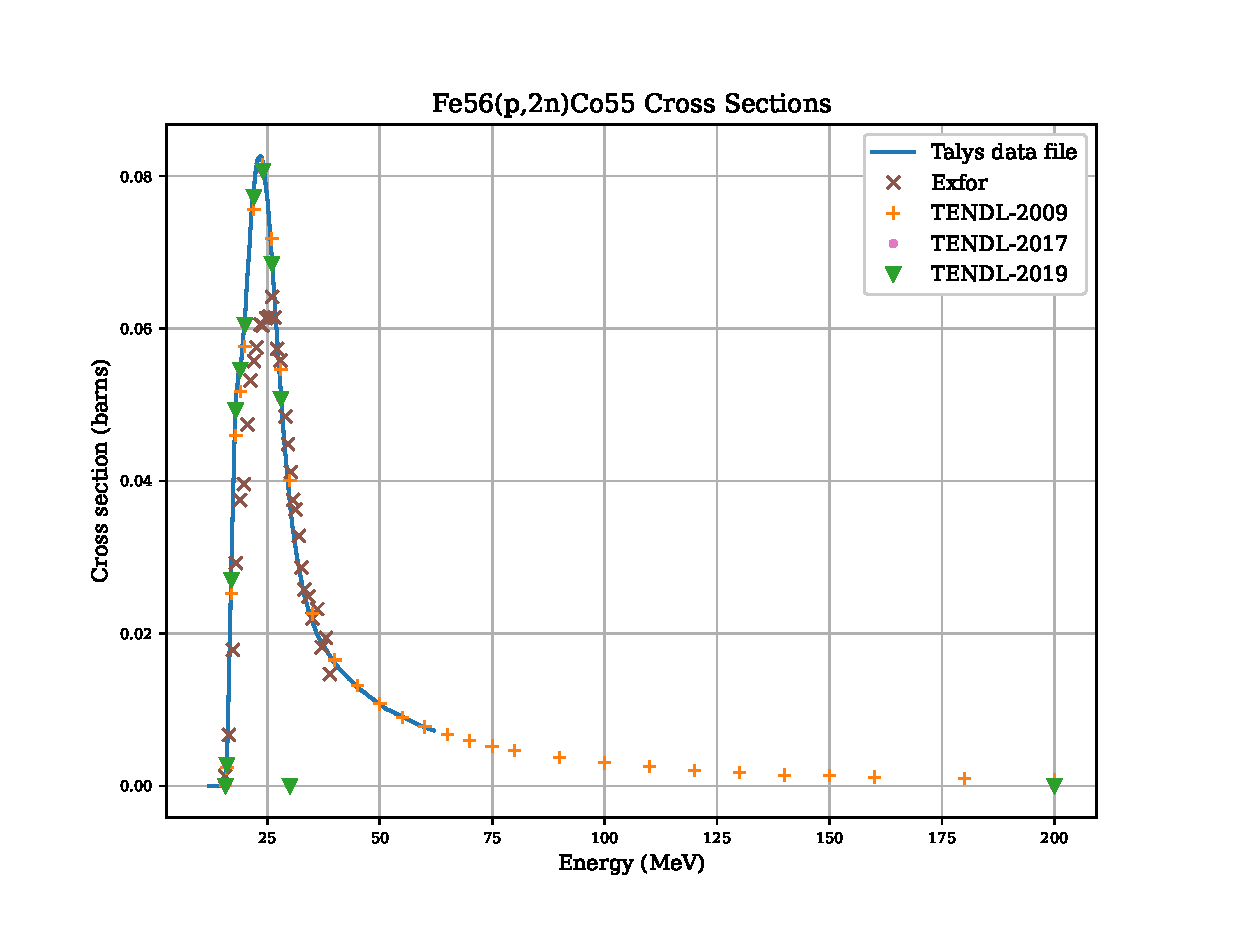
\includegraphics[width=0.7\linewidth]{chapters/activity_code/fe56_co55/Fe56_Co55.eps}
\caption{$Fe56(p,2n)Co55$ cross section data from several sources \cite{tendl2009}\cite{tendl2017}\cite{tendl2019}\cite{exforco55}\cite{talys}}
\label{fig:fe56co55-cross-sections}
\end{figure}
\FloatBarrier

The activity of the sample, in particular due to the radioactivity of ${}^{55}_{27}Co$, was estimated using a number of data sources.  As a consequence of the short beam duration when compared to the half-life of Cobalt-55, any loss during irradiation is ignored in each case.  

The estimations use one set of experimental data, from the \acrshort{exfor} data file, as well as evaluated and calculated data points.  As may be seen in \ref{fig:fe56co55-cross-sections}, all data sets follow a similar path although the peak is slightly lower for the experimental data.  The two most recent TENDL data plots terminate abruptly, but the TENDL-2009 and TALYS calculated data points continue in agreement with one another up to 62MeV, where the calculated points end.

The parameters in relation to the beam current, duration, target material and the gamma intensity were consistent between the estimations.  They are the same parameters as used in the experimental work and are given in table \ref{table:activityestimation1}.

\FloatBarrier
\begin{table}[h]
\begin{center}
\begin{tabular}{c c}
\hline\hline
Parameter & Value\\
\hline\hline
ND/atoms ${}^{56}_{26}Fe$ & $7.4 \times 10^{28}$ \\
ND/atoms ${}^{54}_{26}Fe$ & $4.6 \times 10^{27}$ \\
J/amps & $0.5 \times 10^{-7}$ \\
Q/C & $1.60 \times 10^{-19}$ \\
d/m & $5.0 \times 10^{-4}$ \\
irradiation time/s & $3.0 \times 10^{2}$ \\
Co55 t-half/s & $6.3 \times 10^{4}$ \\
Co55 $\lambda$ & $1.1 \times 10^{-5}$ \\
931KeV Gamma Intensity & $0.75$ \\
\hline\hline
\end{tabular}
\end{center}
\caption{Parameters used to estimate Co55 931KeV gamma activity}
\label{table:activityestimation1}
\end{table}

The 2019 data file ranges up to 30MeV for the ${}^{54}_{26} Fe (p, \gamma) {}^{55}_{27} Co$ and ${}^{56}_{26} Fe (p, 2n) {}^{55}_{27} Co$ reactions.  As the data cuts off at 30MeV, the cross section data for a 28-30MeV proton is used in the estimation.  This results in an over estimate in activity.

A 36MeV proton is expected to lose up to 4-5MeV travelling through a 0.5mm thick Iron target, as seen in figure \ref{fig:fe36mevenergydepth}.  However, in this estimation the ions are assumed to be only 36MeV (or 28MeV, where 36MeV data are unavailable).

\begin{table}[h]
\begin{center}
\begin{tabular}{c c c c c c c}
\hline\hline
 & TENDL 2009 & TENDL 2017 & TENDL 2019 & Exfor & TALYS file & TALYS DB \\
\hline\hline
\multicolumn{7}{c}{${}^{54}_{26}Fe(p,\gamma){}^{55}_{27}Co$}\\
P energy (MeV) & 36 & 28 & 28 & 36 & 36 & 36  \\
XS $\sigma$ (barns) & $1.29 \times 10^{-4}$ & $1.94 \times 10^{-4}$ & $1.94\times 10^{-4}$ & - & $1.33 \times 10^{-4}$ & $1.75 \times 10^{-4}$ \\
Reaction Rate & $9.32 \times 10^{4}$ & $1.40 \times 10^{5}$ & $1.40 \times 10^{5}$ & -  & $9.64 \times 10^{4}$ & $1.27\times 10^{5}$ \\
Activity (Bq) & $1.78 \times 10^{1}$ & $2.69 \times 10^{1}$ & $2.69 \times 10^{1}$ & -  & $1.84 \times 10^{1}$ & $2.43 \times 10^{1}$ \\
Gamma (Bq) & $1.34 \times 10^{1}$ & $2.02 \times 10^{1}$ & $2.02 \times 10^{1}$ & -  & $1.38 \times 10^{1}$ & $1.82 \times 10^{1}$ \\
\multicolumn{7}{c}{${}^{56}_{26}Fe(p,2n){}^{55}_{27}Co$}\\
P energy (MeV) & 36 & 28 & 28 & 36 & 36 & 36  \\
XS $\sigma$ (barns) & $2.13 \times 10^{-2}$ & $5.08 \times 10^{-2}$ & $5.08\times 10^{-2}$ & $2.30\times 10^{-2}$ & $2.00 \times 10^{-2}$ & $2.00 \times 10^{-2}$ \\
Reaction Rate & $2.44 \times 10^{8}$ & $5.81 \times 10^{8}$ & $5.81 \times 10^{8}$ & $2.64 \times 10^{8}$  & $2.29 \times 10^{8}$ & $2.29\times 10^{8}$ \\
Activity (Bq) & $4.67 \times 10^{4}$ & $1.11 \times 10^{5}$ & $1.11 \times 10^{5}$ & $5.04 \times 10^{4}$  & $4.38 \times 10^{4}$ & $4.38 \times 10^{4}$ \\
Gamma (Bq) & $3.50 \times 10^{4}$ & $8.33 \times 10^{4}$ & $8.33 \times 10^{4}$ & $3.78 \times 10^{4}$  & $3.29 \times 10^{4}$ & $3.29 \times 10^{4}$ \\
\hline\hline
\end{tabular}
\end{center}
\caption{Estimation of the Cobalt-55 931KeV gamma activity based on the \acrshort{tendl}-2009\cite{tendl2009}, \acrshort{tendl}-2017\cite{tendl2017}, \acrshort{tendl}-2019\cite{tendl2019} data files, \acrshort{exfor} experimental data \cite{exforco55} and TALYS generated data files\cite{talys}.}
\label{table:activityestimation2}
\end{table}

The largest contribution to the 931KeV gamma is due to the ${}^{56}_{26} Fe (p, 2n) {}^{55}_{27} Co$
reaction, with the ${}^{54}_{26} Fe (p, \gamma) {}^{55}_{27} Co$ reaction being responsible for less than 0.1\% of the gammas.

Out of the estimates calculated, the outliers are those that used data files with a 28 MeV maximum limit, and this is as to be expected.  The final three results are much closer to one another, ranging from 43,800Bq to 50,400Bq for the overall activity and 32,900Bq to 37,800Bq for the rate of emission of Gammas.  The full details including cross sections and reaction rates used are given in table \ref{table:activityestimation2}.


\FloatBarrier


\subsection{Simulating Proton Irradiated Iron with Actvity V1}

The activity code with the derived activity equations was used to calculate the predicted radioactivity (figure \ref{fig:act1top5radioactive}) and predicted gamma lines (figure \ref{fig:act1gammalines}).  A full output file and details of all isotopes and their activities are in Appendix \autoref{chapter:appendix-activity-v1}.

\FloatBarrier
\begin{figure}[!htb]
\minipage{0.49\textwidth}
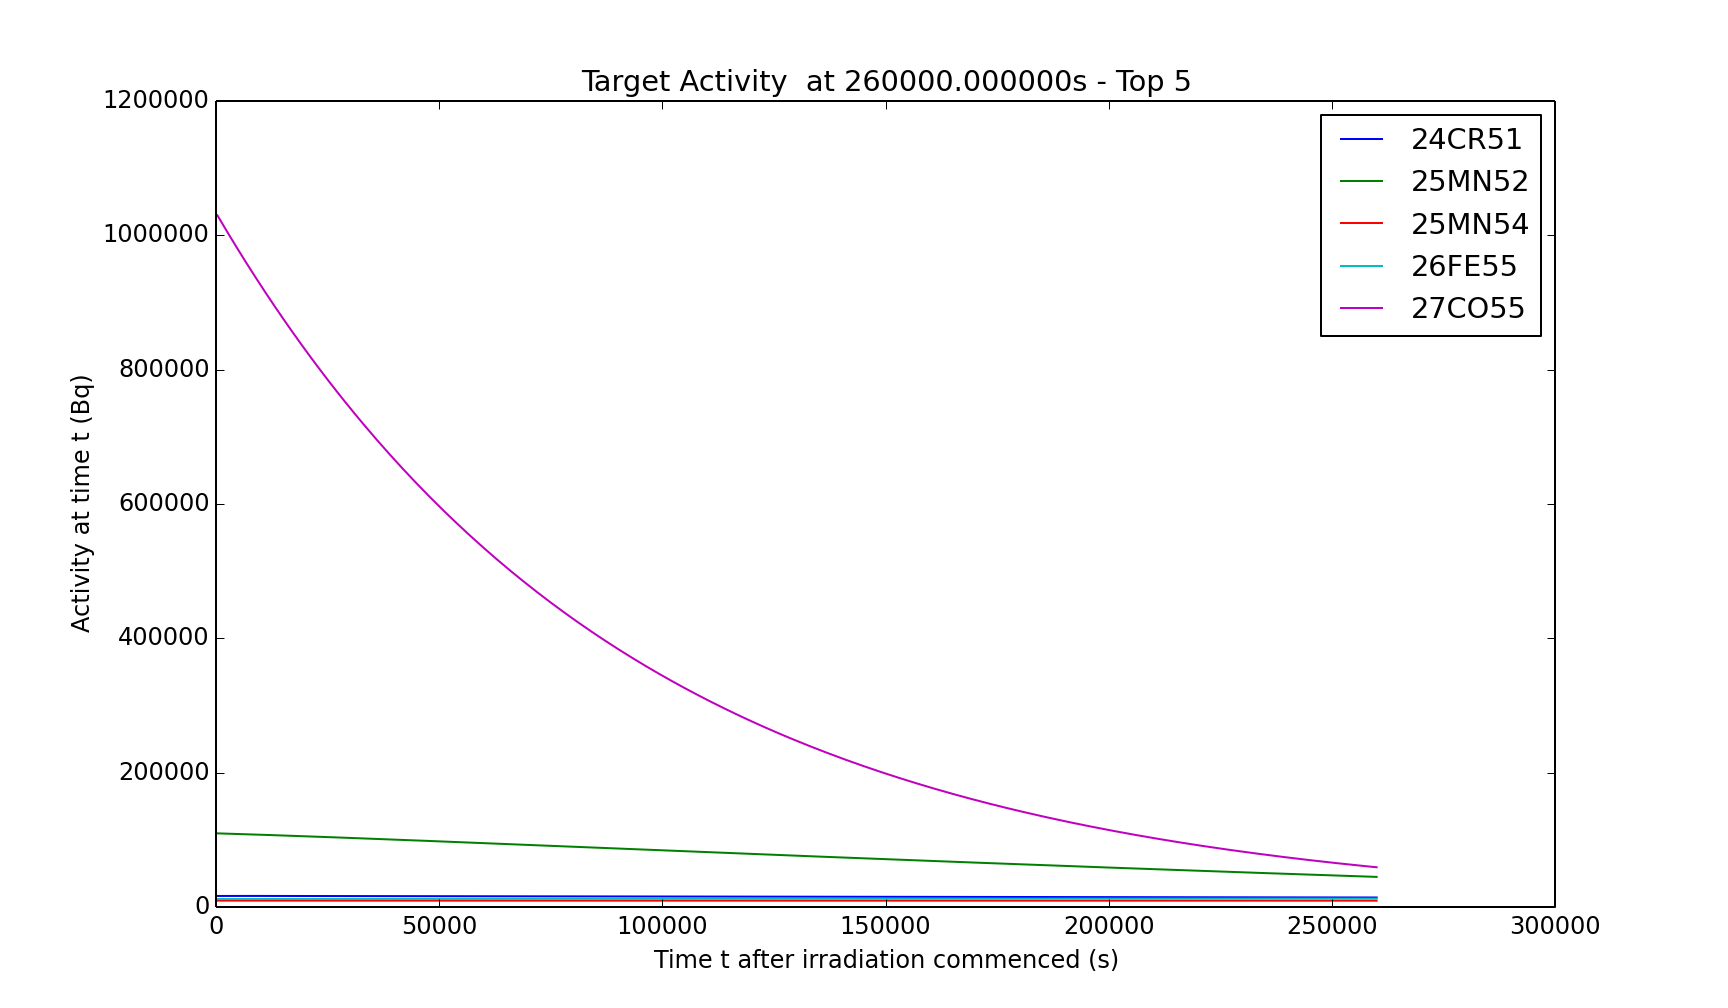
\includegraphics[width=\linewidth]{chapters/activity_code/fe-activity-v1/activityTop5_Fe36MeV.png}
\caption{Isotopes with the top 5 radioactivity plotted over approximately 3 days}
\label{fig:act1top5radioactive}
\endminipage\hfill
\minipage{0.49\textwidth}
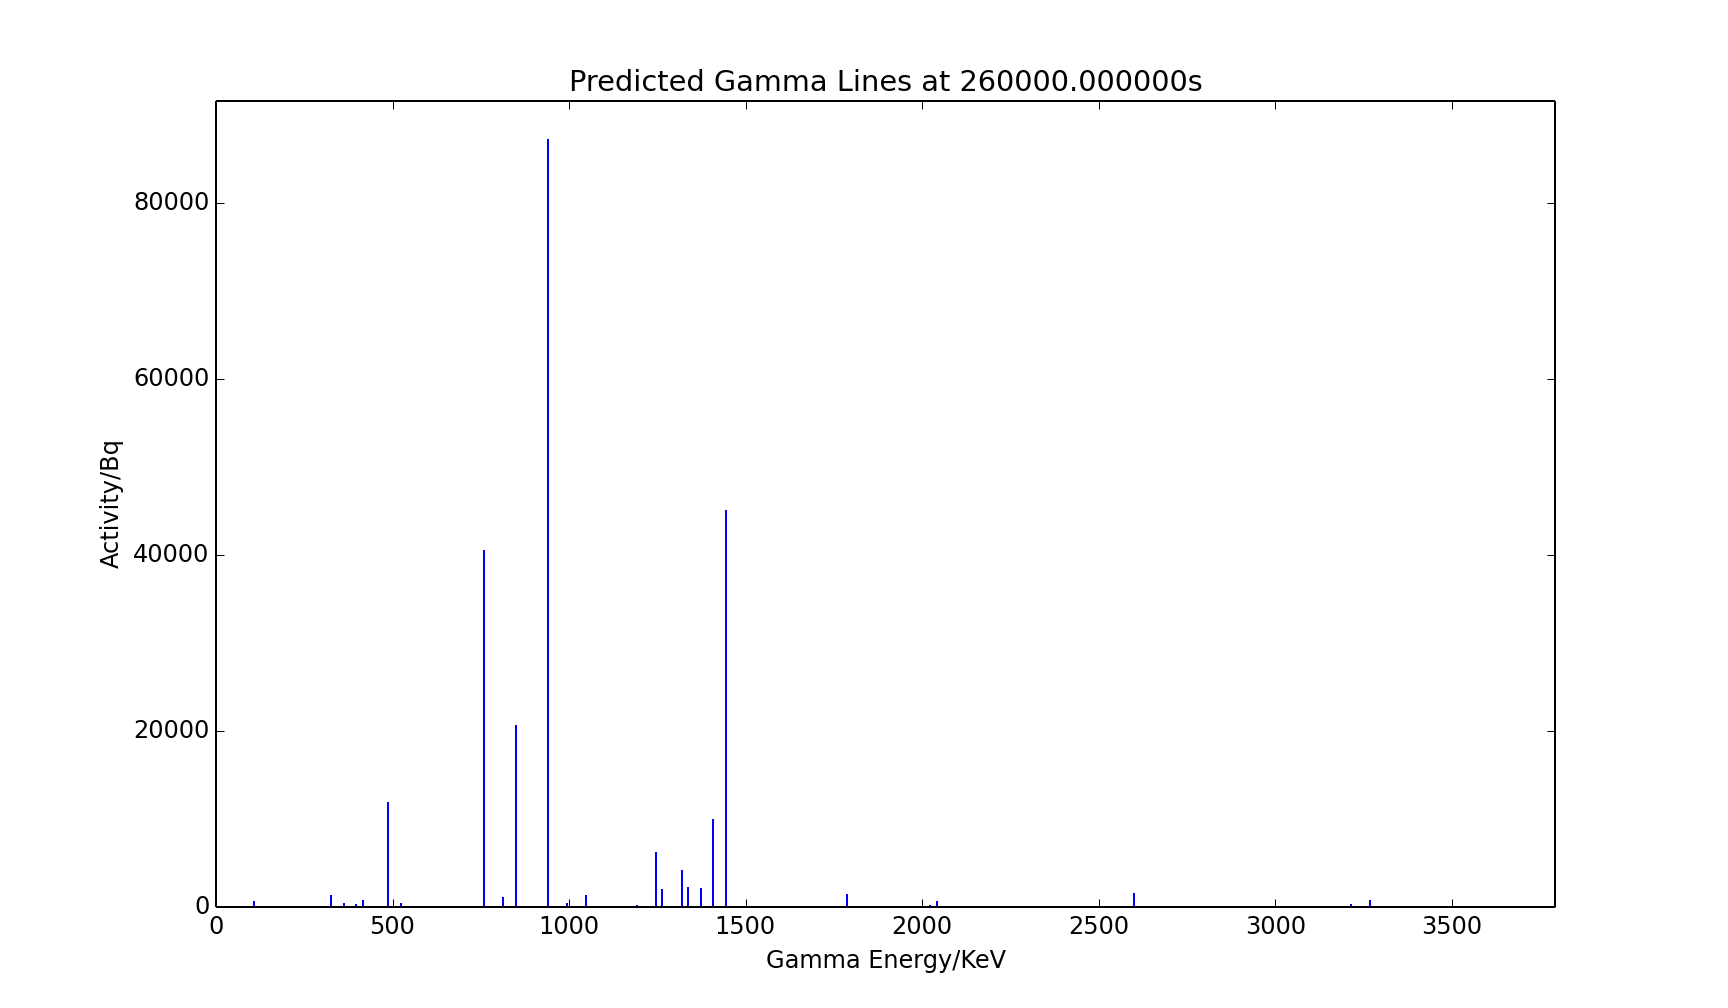
\includegraphics[width=\linewidth]{chapters/activity_code/fe-activity-v1/gammaLines_Fe36MeV.png}
\caption{Predicted gamma lines approximately 3 days after irradiation}
\label{fig:act1gammalines}
\endminipage
\end{figure}
\FloatBarrier

The code predicts a final 931KeV gamma activity of over 59,000 Bq and highlights several other isotopes of interest, including ${}^{52}_{25} Mn$, ${}^{51}_{24} Cr$, ${}^{55}_{26} Fe$ and ${}^{54}_{25} Mn$, all of which have an activity of approximately 10,000 Bq or above.  After 3 days of cooling, the target is predicted to dose an 80KG human, 1 meter away from the target, with $4.0 \times 10^{-11}$ Gy/s (absorbed dose) which is less than the limit for a member of the public ($6.34 \times 10^{-10}$ Si/s, effective dose). 




\subsection{Simulating Proton Irradiated Iron with Actvity V2}

The iron irradiation experiment was modelled using the second version of the activity code.  In this version the entire cross section database was created using the TALYS computer code (\ref{section:activitytalysdb}).  The same decay equations used in version 1 were also used here.

As the iron sample is irradiated a large number of particles (neutrons, protons, deuterons, tritons, helium-3, alphas and gammas) are created.  Whilst the beam is on, these are produced at a rate of more than $10^9$ per second (figure \ref{fig:activity-v2-particle-production}).

As irradiation commences, the isotope of iron responsible for most of the non-particle radiation is ${}^{54}_{26} Fe$, despite having a natural abundance of only 5.8\%.  Two residuals in particular resulting from proton reactions with ${}^{54}_{26} Fe$ are responsible for the activity and these are ${}^{54}_{25}Co$ and ${}^{53}_{26}Fe$.  

\begin{figure}[htb]
\centering
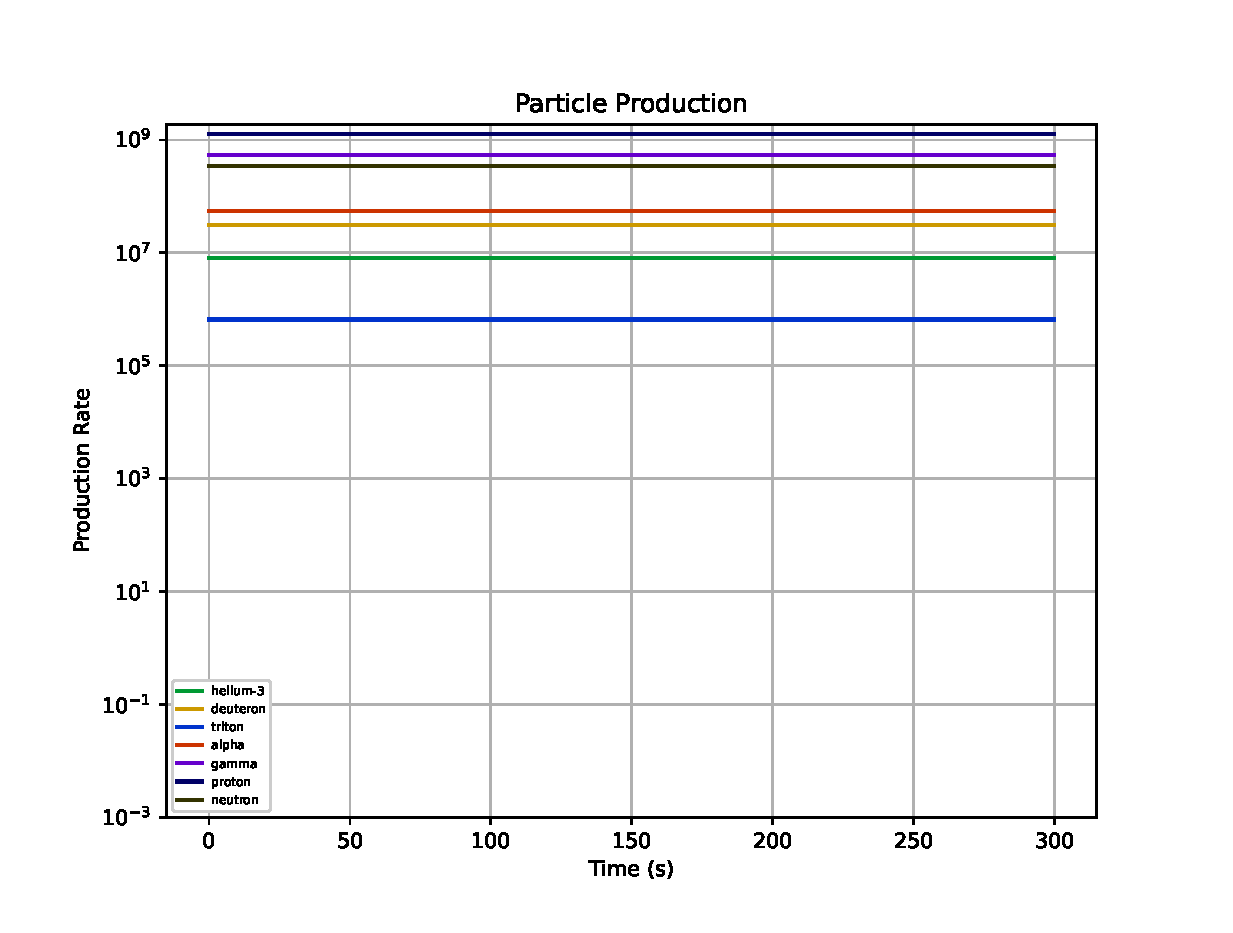
\includegraphics[width=0.5\linewidth]{chapters/activity_code/fe-activity-v2/particle_production_in_beam.eps}
\caption{Particle production rate in beam}
\label{fig:activity-v2-particle-production}
\end{figure}

With a short half life of 0.19 seconds, ${}^{54}_{25}Co$ is responsible for the majority of decays per second within a few seconds of irradiation starting.  However, at this same time the majority of the gamma energy from residual isotopes originates from the decays of ${}^{53}_{26}Fe$ (meta 1) and  ${}^{52}_{25}Mn$ (meta 1).  The average gamma energy per decay of these isotopes is 3.03MeV and 1.42MeV respectively, and this is the reason for such a high contribution towards the gamma energy output (\ref{fig:activity-v2-residual-1}).

By the time the beam is turned off, at 300s, the primary isotope contributing almost 50\% of the decays per second is ${}^{53}_{26}Fe$.  It's contribution to the over all gamma output is still quite low with the main contributor being ${}^{52}_{25}Mn$ (meta 1) as was the case at the start of irradiation (\ref{fig:activity-v2-residual-2}).  This difference between the decays and gamma energy is due to ${}^{53}_{26} Fe$ having an average gamma energy of only 0.18MeV per decay, whereas the metastable ${}^{52}_{25} Mn$ has a much higher average gamma energy per decay of 1.4MeV.

\begin{figure}[htb]
\centering
\begin{subfigure}{0.49\textwidth}
  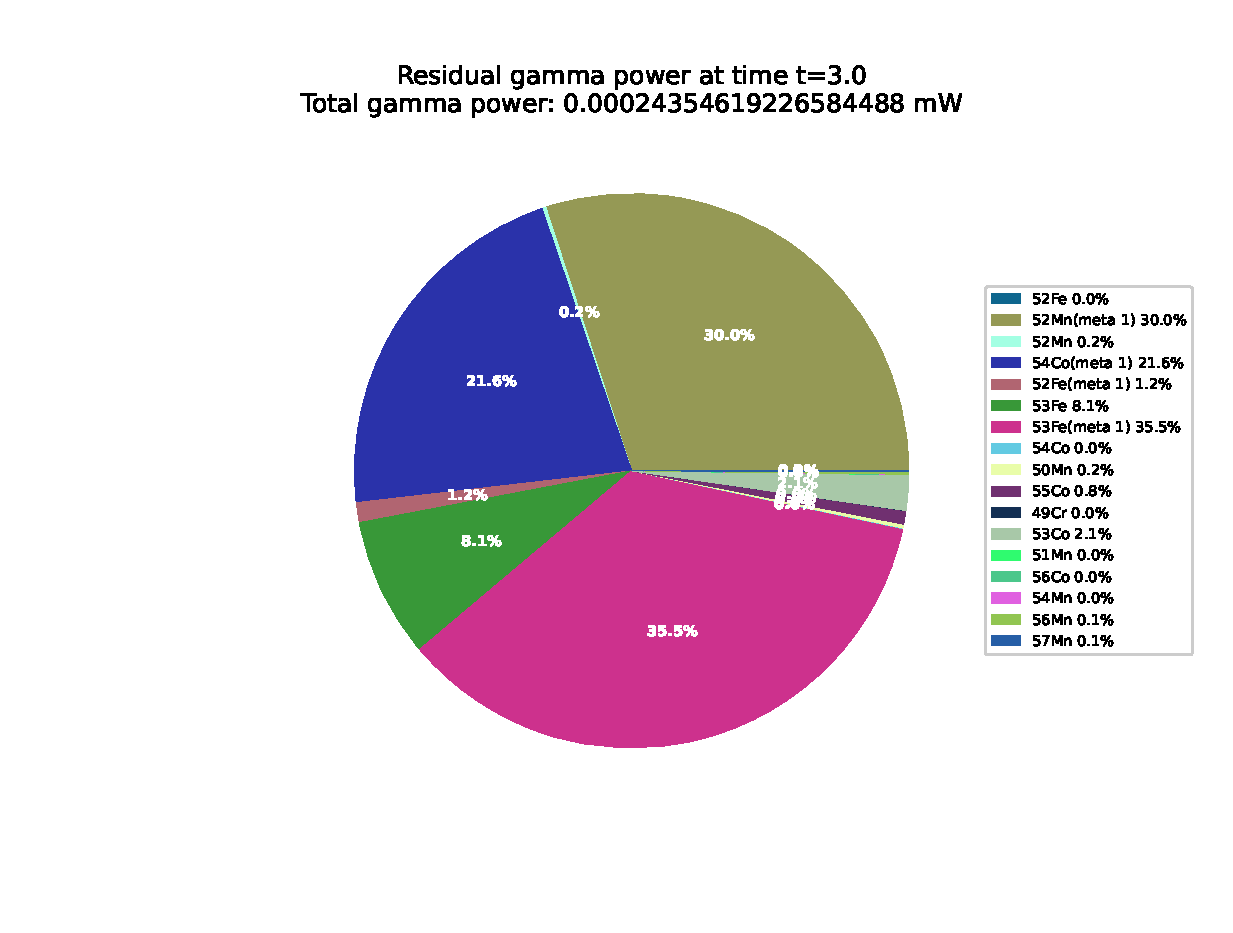
\includegraphics[width=\linewidth]{chapters/activity_code/fe-activity-v2/residual-energy/0001_3.eps}
  \caption{Beam on, t=3.0s}
  \label{fig:activity-v2-residual-1}
\end{subfigure}\hfil % <-- added
\begin{subfigure}{0.49\textwidth}
  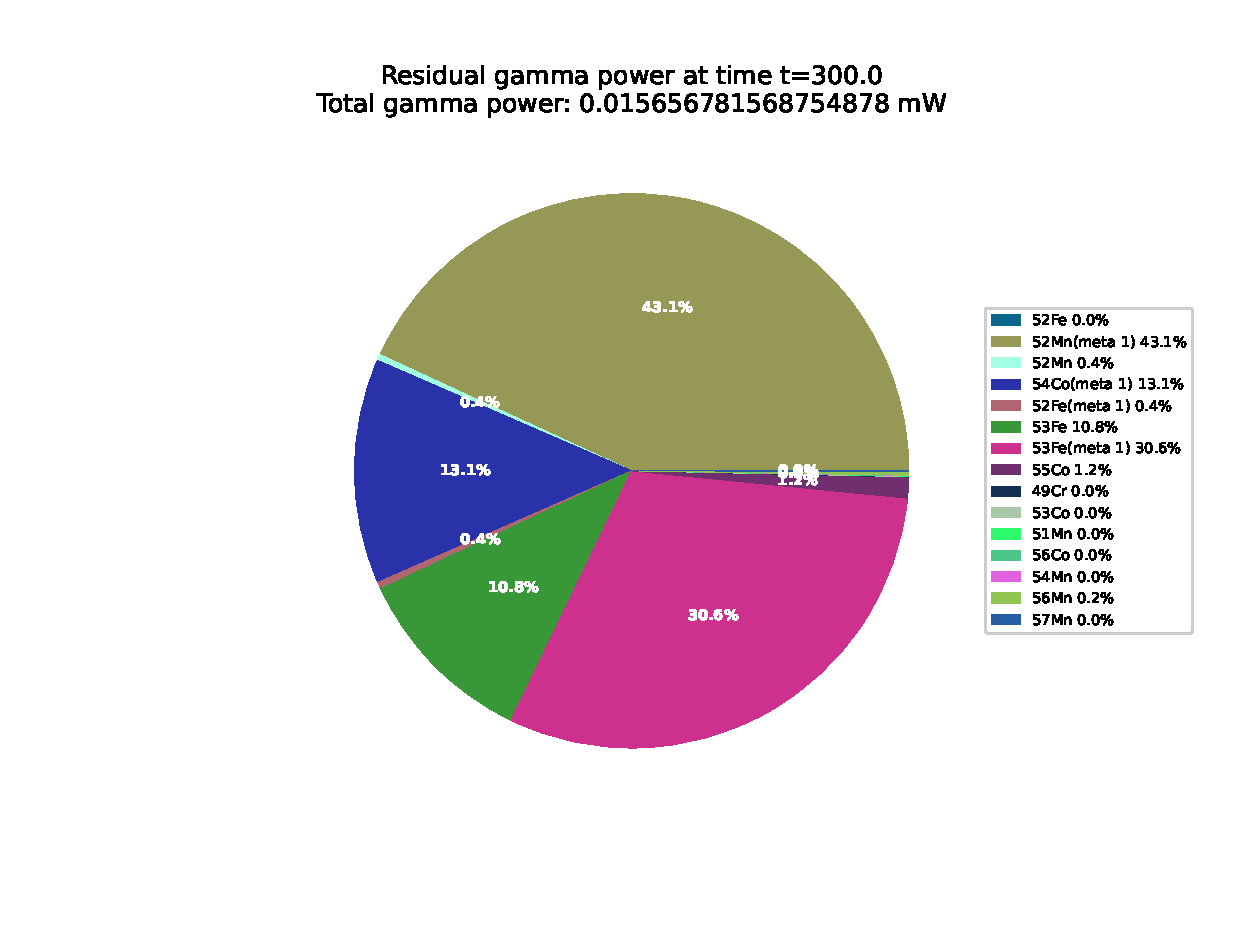
\includegraphics[width=\linewidth]{chapters/activity_code/fe-activity-v2/residual-energy/0100_300.eps}
  \caption{Beam on, t=300.0s}
  \label{fig:activity-v2-residual-2}
\end{subfigure}
\caption{Gamma output of residual isotopes, by isotope, at the start and end of irradiation}
\label{fig:activity-v2-residual-a}
\end{figure}

Once the beam is turned off, those isotopes with a very short half life decay away quickly.  After 1 day of cooling, the isotopes responsible for activity in the sample are very different.  With a half life of less than 10 minutes, the ${}^{53}_{26}Fe$ will have decayed to nothing as would have the ${}^{53}_{26}Fe$ (meta 1) and ${}^{52}_{25}Mn$ (meta 1).  At this time, the isotope with the highest contribution to decays per second will be ${}^{55}_{27}Co$, but with a half-life of 17.53 hours it does not remain the largest contributor.  It is also responsible for more than half of the gamma power output at this time as well (\ref{fig:activity-v2-residual-3}).

At the end of the experiment, the time at which the experimental gamma readings were taken ($2.6 \times 10^5$s), the largest contributor to both decays per second and gamma energy output per second is the ${}^{52}_{25}Mn$ isotope (\ref{fig:activity-v2-residual-4}).

\begin{figure}[htb]
\centering
\begin{subfigure}{0.49\textwidth}
  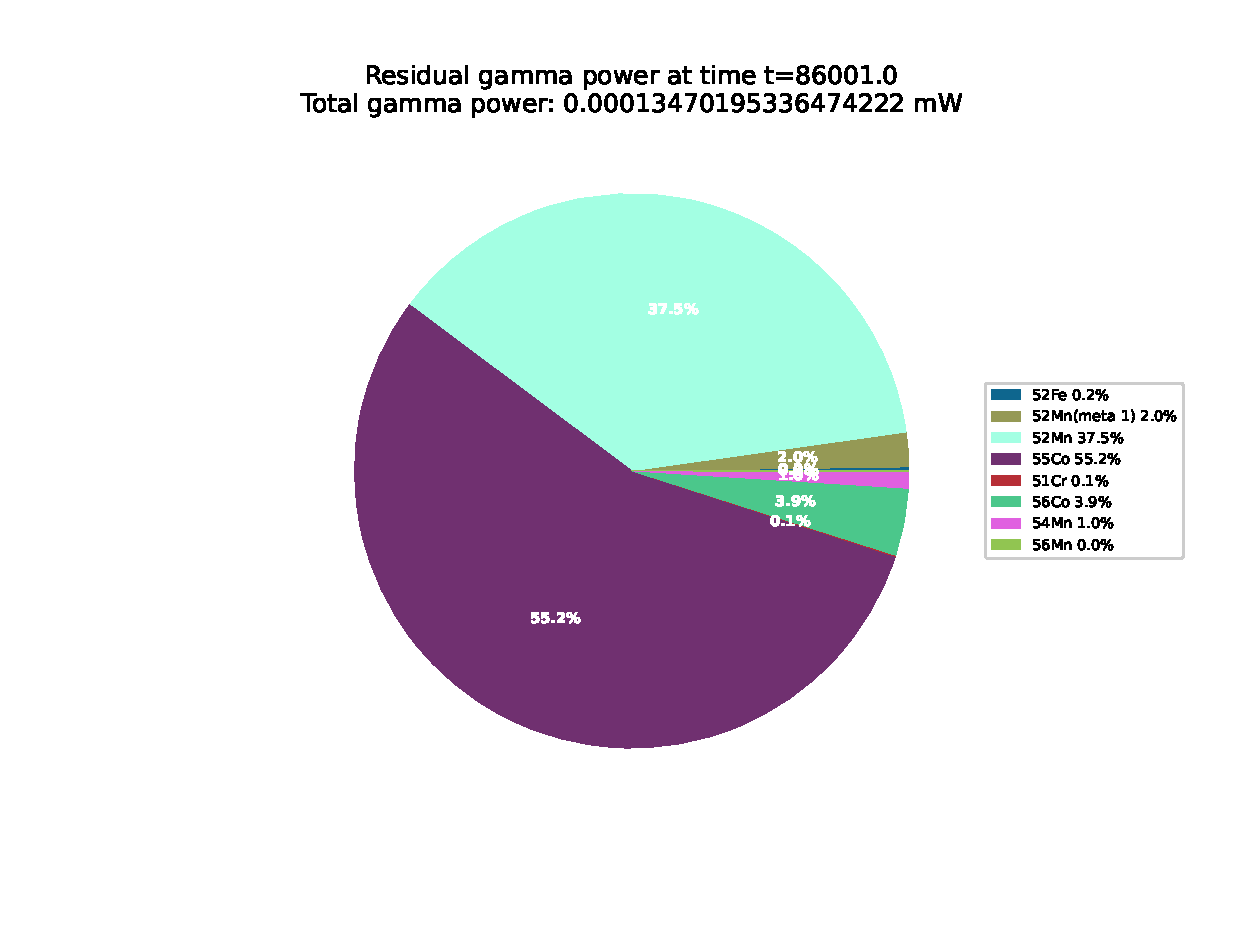
\includegraphics[width=\linewidth]{chapters/activity_code/fe-activity-v2/residual-energy/0166_86001.eps}
  \caption{Beam off, t=86001.0s}
  \label{fig:activity-v2-residual-3}
\end{subfigure}\hfil % <-- added
\begin{subfigure}{0.49\textwidth}
  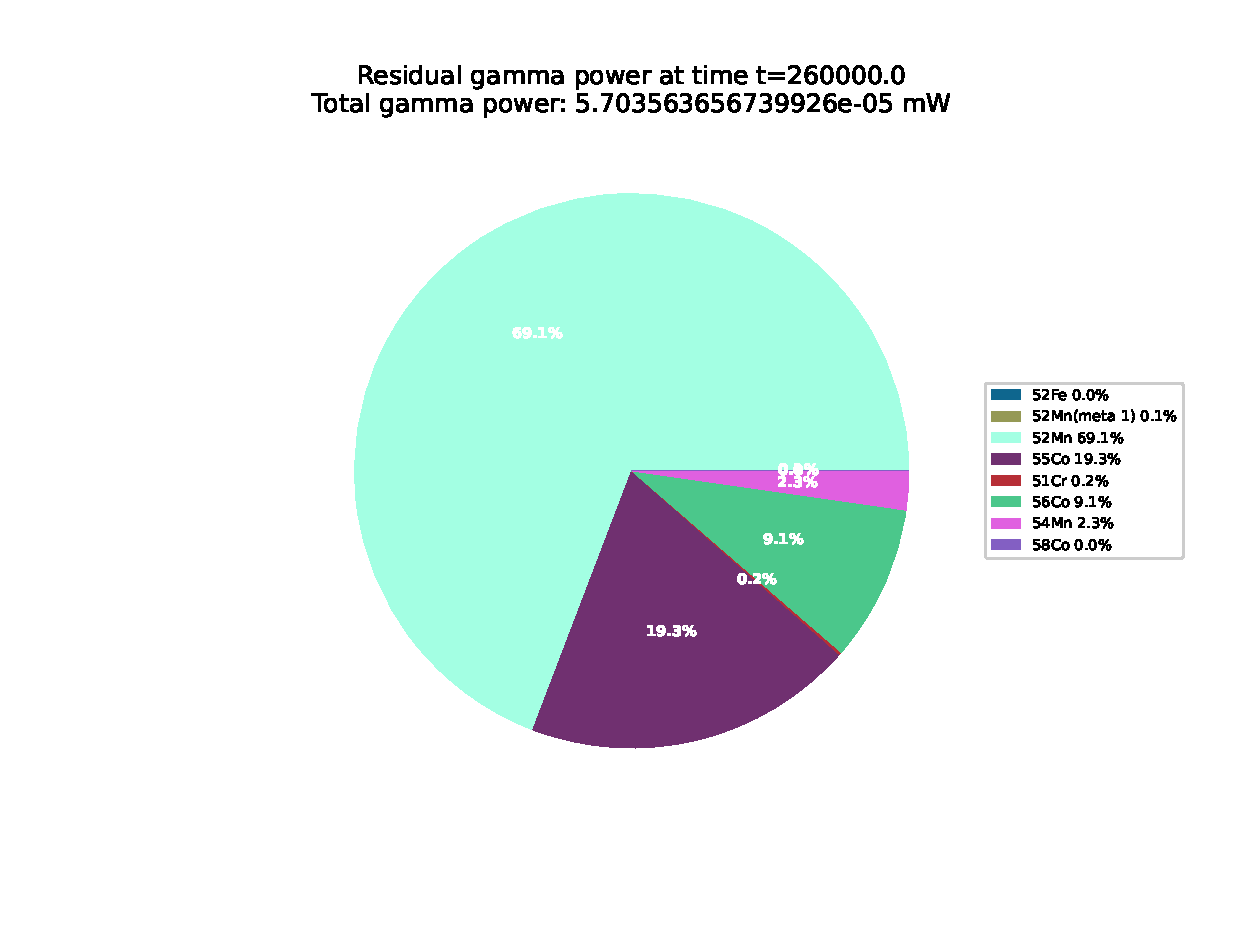
\includegraphics[width=\linewidth]{chapters/activity_code/fe-activity-v2/residual-energy/0300_260000.eps}
  \caption{{Beam off, t=260000.0s}}
  \label{fig:activity-v2-residual-4}
\end{subfigure}
\caption{Residual isotope power output, by residual, once beam is off.}
\label{fig:activity-v2-residual-b}
\end{figure}

The computer code also calculates the predicted gamma lines as time goes by.  The gamma lines become more prominent whilst the ion beam is irradiating the target to a maximum activity at 300 seconds.  The three most active gammas at this point are computed to be 1.43MeV, 378KeV and 701KeV.  The 1.43MeV gamma is released by the decay of the metastable isotope ${}^{52}_{25}Mn$ (meta 1) and is emitted at a rate of $2.9 \times 10^7$Bq.  The 377KeV and 791KeV gammas are emitted by ${}^{53}_{26}Fe$ and ${}^{53}_{26}Fe$ (meta 1) respectively having emission rates of $2.4 \times 10^7$Bq and $9.7 \times 10^{6}$Bq.

As noted previously, the isotopes responsible for change over time and in particular when the source, the proton beam, is removed.  Following a day of cooling the 931KeV gamma from ${}^{55}_{27}Co$ will have an activity of approximately $2.9 \times 10^5$Bq and this is accompanied by another gamma of similar energy.  This is the 935KeV gamma from the decay of ${}^{52}_{25}Mn$.  At this point in time the activity of the 935KeV gamma is less than that of the 931KeV gamma with an activity of $9.49 \times 10^4$Bq.  In addition, the ${}^{52}_{25} Mn$ will also emit a 1.43 MeV gamma at a similar rate calculated to be $1.0 \times 10^5$Bq.  With half lives of 17.5 hours for ${}^{55}_{27} Co$ and 134 hours for ${}^{52}_{25} Mn$ it is clear that, at some point, the activity of the 931KeV gamma will drop below that of the 935KeV gamma.

\FloatBarrier
\begin{figure}[!htb]
\centering
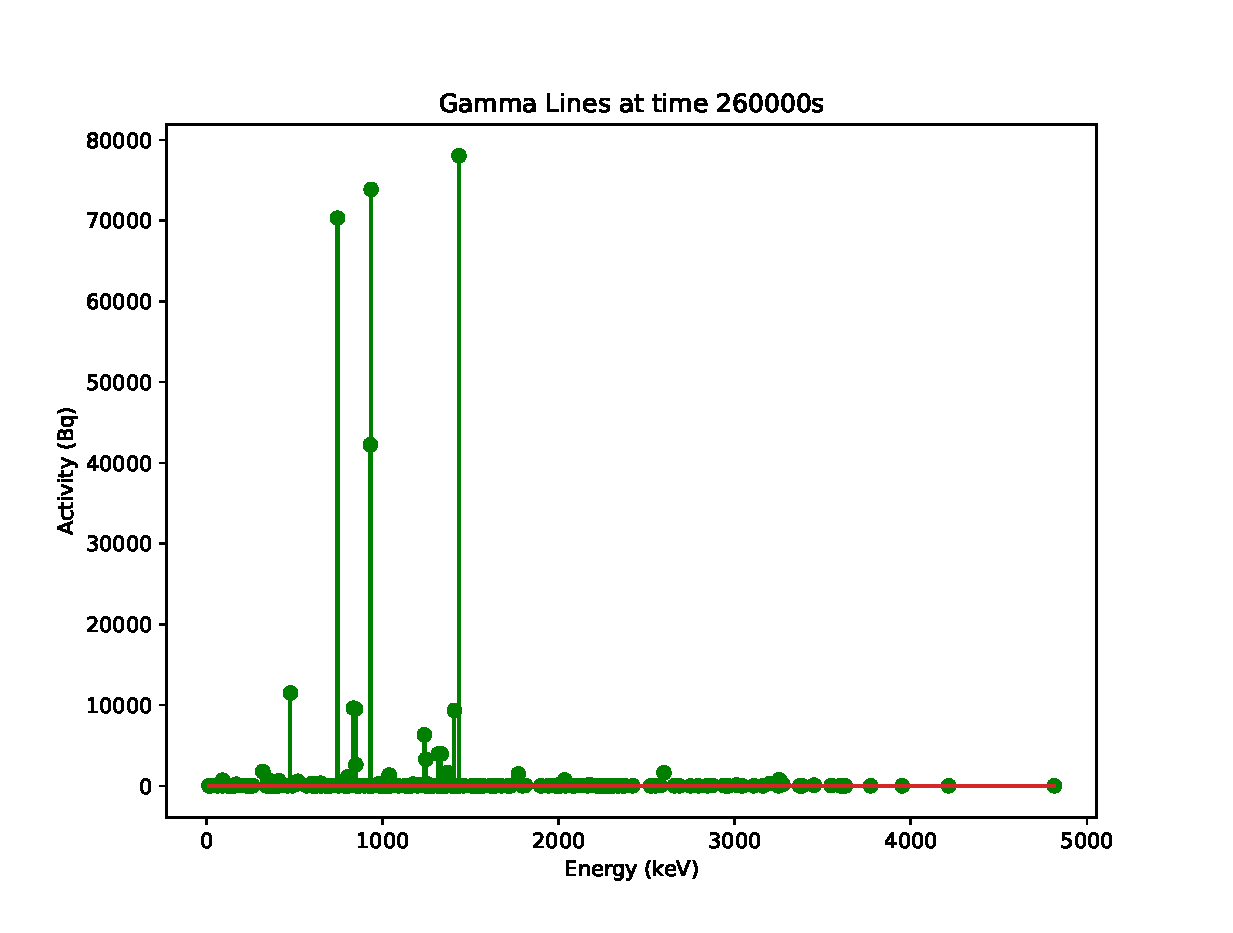
\includegraphics[width=0.6\linewidth]{chapters/activity_code/fe-activity-v2/gammas/0300_260000.eps}
\caption{Expected gamma lines by the end of the experiment (3 days)}
\label{fig:act2totalactivity}
\end{figure}

At the end time of the simulated experiment, $2.6 \times 10^5$s, the activity of the 931KeV Gamma is predicted to have dropped to just over 42,000Bq.  It's neighbour, the 935KeV Gamma, will have an activity almost double, with 74,000 decays per second (figure \ref{fig:act2totalactivity}).  The full results calculated by this code are included in the appendix, chapter \ref{chap:appendix-activity-v2}.  

The prediction of such a large neighbouring Gamma does raise a question where the experimental value is concerned.  It may be that, due to the resolution of the Gamma detector, the measured peak is the sum of both the 931KeV and 935KeV Gamma.  Ideally the detector would be calibrated for a smaller range about that peak and the experiment would be repeated.
 

\subsection{Comparing Experimental Results with Calculated Values}

The estimation is cruder and does not take into account the details of the loss of energy of the projectile as it passes through the target.  It also does not take into account the creation of ${}^{55}_{27} Co$ through other reactions.  It gives a lower value of activity that the computer codes and the experimentally measured value (table \ref{table:activityResultsCompared}).

\begin{table}[h]
\begin{center}
\begin{tabular}{c c}
\hline\hline
Value source & Co-55 Gammas/second at approximately 3 days \\
\hline\hline
Experimental & $4.4\times10^4 +/- 1.05 \times 10^3$ \\
TENDL-2009 & $3.5\times10^4$ \\
Activity V1 & $5.9\times10^4$ \\
Activity V2 & $4.2\times10^4$ \\
\hline\hline
\end{tabular}
\end{center}
\caption{Comparison of proton irradiated iron Co55 931KeV gamma rates}
\label{table:activityResultsCompared}
\end{table}




%%% With the experimental work, the resolution of the detector and software is not that fine as to bin 935KeV counts in with the 931KeV count when integrating counts.


\FloatBarrier


\section[100DPA Predicted Activity]{Predicted Activity for 100DPA Irradiated Iron}

\Acrlong{gen4} reactors are required to withstand 100-150DPA over the lifetime of the plant, which may span 30 years or more.  The Scanditronix cyclotron is capable of creating a 60 microamp beam and, due to the small area (and volume of material) this may be concentrated on, it is able to create high damage rates over a shorter period of time.

The Activity V2 code was used to calculate how radioactive a 100DPA iron sample would be after irradiation at the maximum current setting of 60 microamps.  The simulated target is 0.5mm thick, pure iron and the beam is protons and has an area of $64mm^2$.  The projectile fluence is $3.75 \times 10^{14}$ protons per second, and the number of atoms within the volume of iron are $2.56 \times 10^{21}$.  Five different energy settings were used (5MeV, 10MeV, 15MeV, 20MeV, 25MeV) and the vacancies per ion as well as the ion trajectories were generated by \acrshort{srim}.

\FloatBarrier
\begin{table}[h]
\begin{center}
\begin{tabular}{c c c c c c c}
\hline\hline
                     & 5MeV & 10MeV & 15MeV & 20MeV & 25MeV & 30MeV \\
\hline\hline
\acrshort{vpi}       & 38.5  & 58.8  & 51.0  & 23.7   & 20.2  &  12.8  \\
\acrshort{dpa}/year  & 178   & 272   & 236   & 109    & 93    &  59    \\
Days for 100 DPA     & 205   & 134   & 155   & 333    & 391   &  617   \\
Damage Depth (mm)    & $<$0.1  & 0.25  & 0.5+  & 0.5+   & 0.5+  &  0.5+  \\
Activity\textsuperscript{1} (Bq)        & ${2.27} \times 10^{6}$  & ${7.32} \times 10^{8}$  & ${2.55} \times 10^{9}$  & ${3.66} \times 10^{9}$  & ${4.10} \times 10^{9}$ & ${4.88} \times 10^{9}$ \\    
Gamma Output\textsuperscript{1} (mW)    & ${9.44} \times 10^{-5}$  & ${3.87} \times 10^{-1}$  & ${1.32} \times 10^{0}$  & ${1.29} \times 10^{0}$  & ${6.05} \times 10^{-1}$ & ${5.74} \times 10^{-1}$ \\ 
Activity\textsuperscript{2} (Bq)        & ${2.14} \times 10^{6}$  & ${6.86} \times 10^{8}$  & ${2.35} \times 10^{9}$  & ${3.08} \times 10^{9}$  & ${2.82} \times 10^{9}$ & ${3.52} \times 10^{9}$ \\    
Gamma Output\textsuperscript{2} (mW)    & ${8.85} \times 10^{-5}$  & ${3.64} \times 10^{-1}$  & ${1.24} \times 10^{0}$  & ${1.16} \times 10^{0}$  & ${3.63} \times 10^{-1}$ & ${2.94} \times 10^{-1}$ \\ 
\hline\hline
\end{tabular}
\end{center}
\caption{Comparison of proton irradiated iron up to 100DPA at a range of proton energies.  The first set of measurements\textsuperscript{1} are calculated values at the point the proton beam is turned off.  The second set\textsuperscript{2} are calculated after 1 week of cooling.}
\label{tab:activitydpairon}
\end{table}

In each case the sample was irradiated close to saturation.  Doubling the irradiation time would not be expected to significantly increase the activity, as sufficient time (in each case) is given for the radioactive isotopes being created to balance those decaying away. 

It is clear to see from the predicted activities in table \ref{tab:activitydpairon} that the higher energy beams would take longer to reach 100DPA, as they pass through the target leaving at a high energy, whilst also irradiating the target several orders of magnitude more than 5MeV and 10MeV.

The Coulomb potential between a proton and an iron nucleus, at the combined nuclear radius of both, is approximately 6.5MeV (eq. \ref{eq:coulombbarrier} and eq. \ref{eq:nuclearsize}).  Unlike neutrons radiation, protons need to overcome the Coulomb repulsion and this explains the relatively low radioactive activation by the 5MeV beam.  

\begin{figure}[htb]
\centering
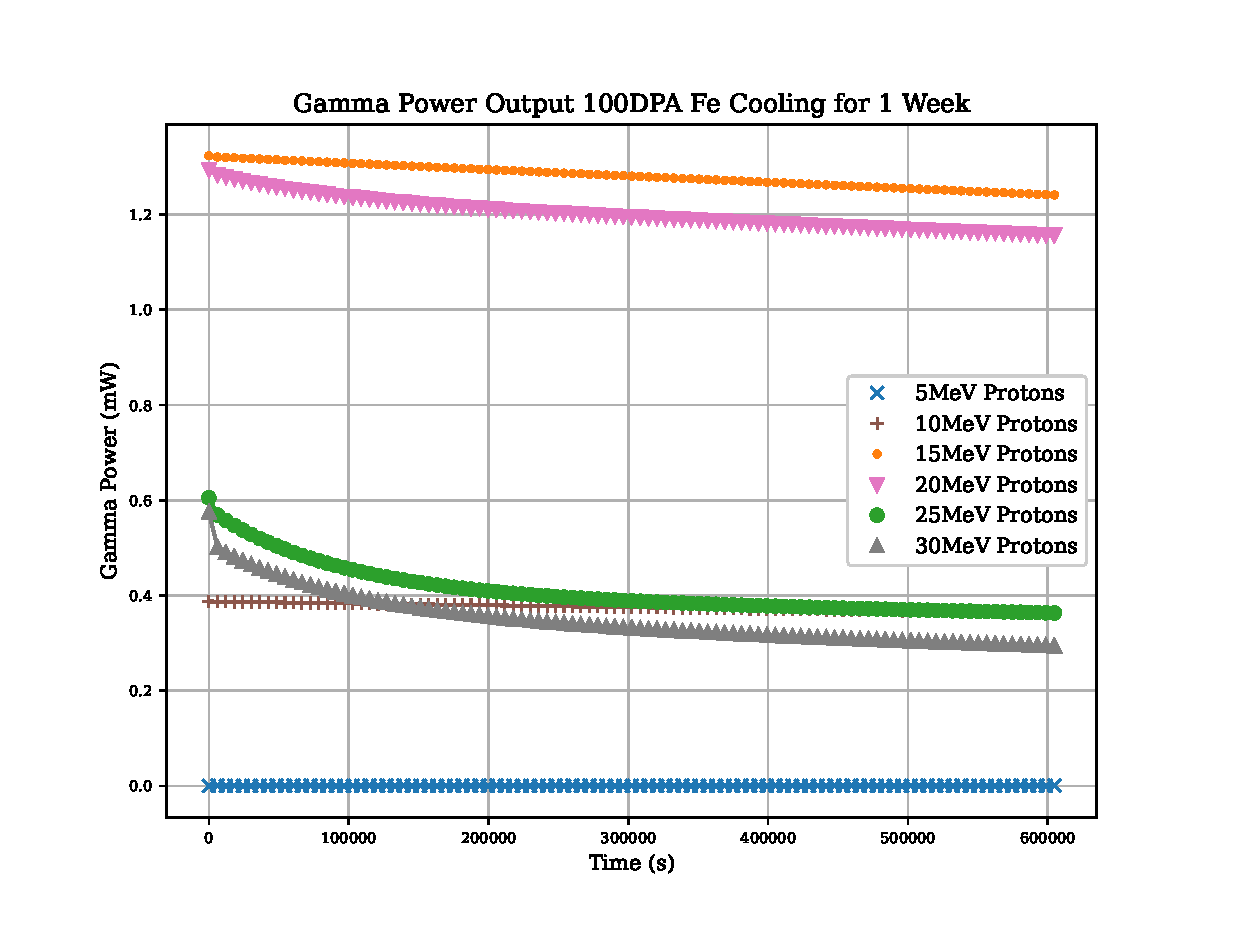
\includegraphics[width=0.7\linewidth]{chapters/activity_code/fe_100dpa/cooling.eps}
\caption{Change in isotope gamma output over time with proton beam off.}
\label{fig:activity-v2-residual-b}
\end{figure}

The predominant isotope responsible for radiation in the 5MeV sample is expected to be ${}^{58}_{27}Co$, and with a half life of 77 days this will remain radioactive for a substantial amount of time (relative to testing by irradiating, cooling then testing the material).

For the 10-20MeV irradiated samples the primary isotope responsible for the radiation is ${}^{56}_{27}Co$, and its contribution to the total gamma output in terms of power ranges from 95\% to 99\%.  This isotope has a similarly long half life, relative to the testing cycle, of 71 days.  Depending upon the volume of material being irradiated, this could lead to problems whereby the sample may need to cool for months to reach a safe activity to handle.

As higher energy protons are used to damage the sample a wider range of reaction possibilities become more likely including that leading to both ${}^{52}_{25}Mn$ and ${}^{52}_{25}Mn (meta 1)$.  By the end of irradiation a large percentage of radioactivity is due to these isotopes (28.6\% for 25MeV protons and 42.8\% for 30MeV protons).  The half life of ${}^{52}_{25}Mn$ and ${}^{52}_{25}Mn (meta 1)$ are short, being 5.6 days and 21 minutes respectively, and will decay away leaving ${}^{56}_{27}Co$ as the main contributor to radiation once again.

Detailed plots resulting from this Activity V2 simulation are in appendix \ref{appendix:ironirradiation}.





\section{Proton Irradiated Molybdenum}

A colleague at the University of Birmingham, John Hewett, irradiated several samples of Molybdenum for materials testing and throughout this the activity of the Molybdenum was measured by the department's HPGe detector\cite{johnhewett}.  Similar to the Iron sample, thin sheets of Molybdenum were irradiated using a beam line from the cyclotron.


\subsection[Experimental Irradiation - Molybdenum]{Molybdenum Experimental Irradiation Results}

A thin 49 micrometer sheet of pure Molybdenum was irradiated with a 13MeV proton beam for 19 seconds at a current of 0.5 microamps.  The beam area on the target was $50mm^2$.  A thick 506 micrometer sheet of the same was also irradiated, but this time a higher beam current of  5 microamps and a duration of 1,500s.

The detector was calibrated to detect energies in the range covering 0MeV to 1.2MeV and several measurements were taken for each sample.  For the thick target the total gamma activity was measured as 16MBq at 3 days (14MBq for gammas above 200KeV) and 7.1MBq at 7 days (6.6MBq for gammas greater than 200KeV).

\begin{figure}[htb]
\centering
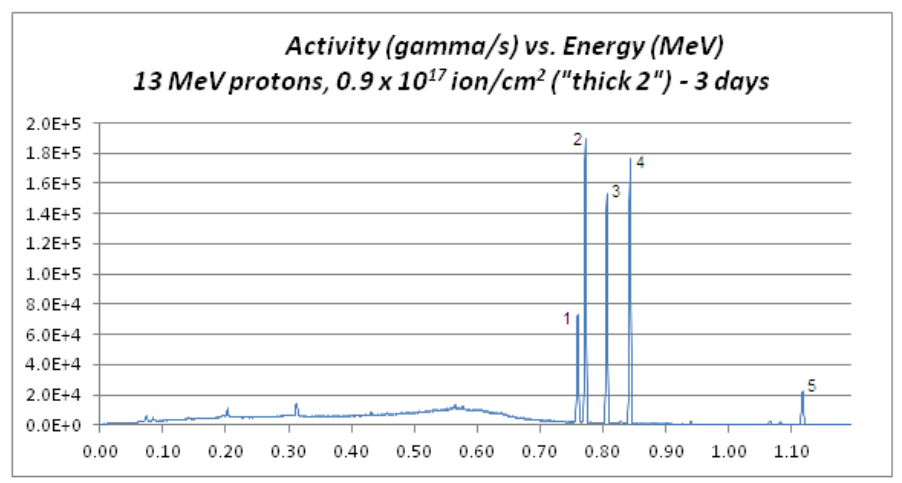
\includegraphics[width=0.7\linewidth]{chapters/activity_code/mo-john-hewett/john_mo_results.png}
\caption{Proton irradiated Molybdenum gamma activity measured by colleague John Hewett}
\label{fig:john-hewett-mo}
\end{figure}

A full gamma spectra was also recorded for the thick sample by gamma peak at three days.  The isotopes responsible for the five most prominent peaks at this point were ${}^{95}_{43}Tc$ (half life of 20 hours\cite{jeff311}) and ${}^{96}_{43}Tc$ (half life of 4.28 days\cite{jeff311}).  The results measured and interpolated by my colleague are given in figure \ref{fig:john-hewett-mo} and table \ref{table:johnhewettresults}.

\FloatBarrier
\begin{table}[h]
\begin{center}
\begin{tabular}{c c c c c c}
\hline\hline
Peak & Energy (KeV) & Isotope & Gamma Intensity & Activity (Bq) & Measured Energy (KeV)\\
\hline\hline
1 & 766 & ${}^{95}_{43}Tc$ & 93.82\% & $5.118 \times 10^{5}$ & 763 \\
2 & 778 & ${}^{96}_{43}Tc$ & 99.76\% & $1.355 \times 10^{6}$ & 776 \\
3 & 813 & ${}^{96}_{43}Tc$ & 82.00\% & $1.155 \times 10^{6}$ & 810 \\
4 & 850 & ${}^{96}_{43}Tc$ & 97.57\% & $1.386 \times 10^{6}$ & 847 \\
5 & 1127 & ${}^{96}_{43}Tc$ & 15.16\% & $2.103 \times 10^{5}$ & 1123 \\
\hline\hline
\end{tabular}
\end{center}
\caption{Gamma emissions measured from a 0.5mm thick sample of Molybdenum irradiated with 13MeV protons at 5 microamps for 1,500 seconds}
\label{table:johnhewettresults}
\end{table}



\subsection{Estimating the Activity of Proton Irradiated Molybdenum}
\label{section:estimatingmoactivity}

The gamma activity of the 0.5mm thick molybdenum target will be estimated.  The generated data are compared to a number of experimental data sources through \acrshort{exfor}.

Naturally occurring Molybdenum is made up of four stable isotopes, two \gls{obsstable} isotopes, ${}^{92}_{42}Mo$ and ${}^{98}_{42}Mo$ and one unstable isotope, ${}^{100}_{42}Mo$, with an extremely long half life of $9.9 \times 10^19$ years (figure \ref{fig:john-hewett-mo}).

\begin{figure}[htb]
\centering
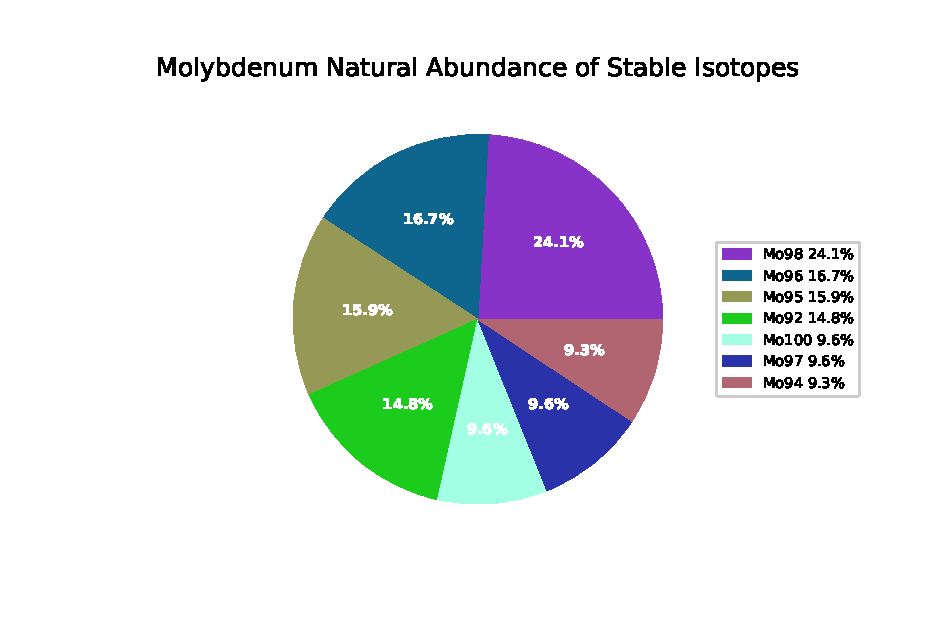
\includegraphics[width=0.5\linewidth]{chapters/activity_code/mo-john-hewett/mo.eps}
\caption{Isotopes in naturally occurring Molybdenum}
\label{fig:john-hewett-mo}
\end{figure}

There are five reactions of particular interest that are predicted to create radioactive isotopes at the highest rate.  Two of the residual isotopes were identified in the experimental work and the reactions responsible are the first two of the five listed below.

\begin{itemize}
\item ${}^{95}_{42}Mo (p, n) {}^{95}_{43}Tc$
\item ${}^{96}_{42}Mo (p, n) {}^{96}_{43}Tc$
\item ${}^{96}_{42}Mo (p, n) {}^{96}_{43}Tc$ (meta 1)
\item ${}^{97}_{42}Mo (p, n) {}^{97}_{43}Tc$
\item ${}^{94}_{42}Mo (p, n) {}^{94}_{43}Tc$
\end{itemize}

The isotope ${}^{95}_{43}Tc$ produced four measurable gamma activities, and these gamma decay rates will be estimated using cross section data available from \acrshort{tendl} and \acrshort{exfor}.  The cross sections have been measured experimentally, with their results published, by four groups since the 1970s.  Whilst there are discrepancies, the total cross section predicted by the TALYS code fits well with the \acrshort{tendl}-2019 database and measurements by Lamere\cite{molamere} and Flynn\cite{moflynn}.  The lower energy cross sections of Hogan\cite{mohogan} do not match as well but the higher energy reactions(30MeV+) are a closer match.  Finally cross section measurements by Levkovski\cite{molevkovski} are slightly larger near to the peak values, but on the whole match well with the TALYS computed values.

\begin{figure}[htb]
\centering
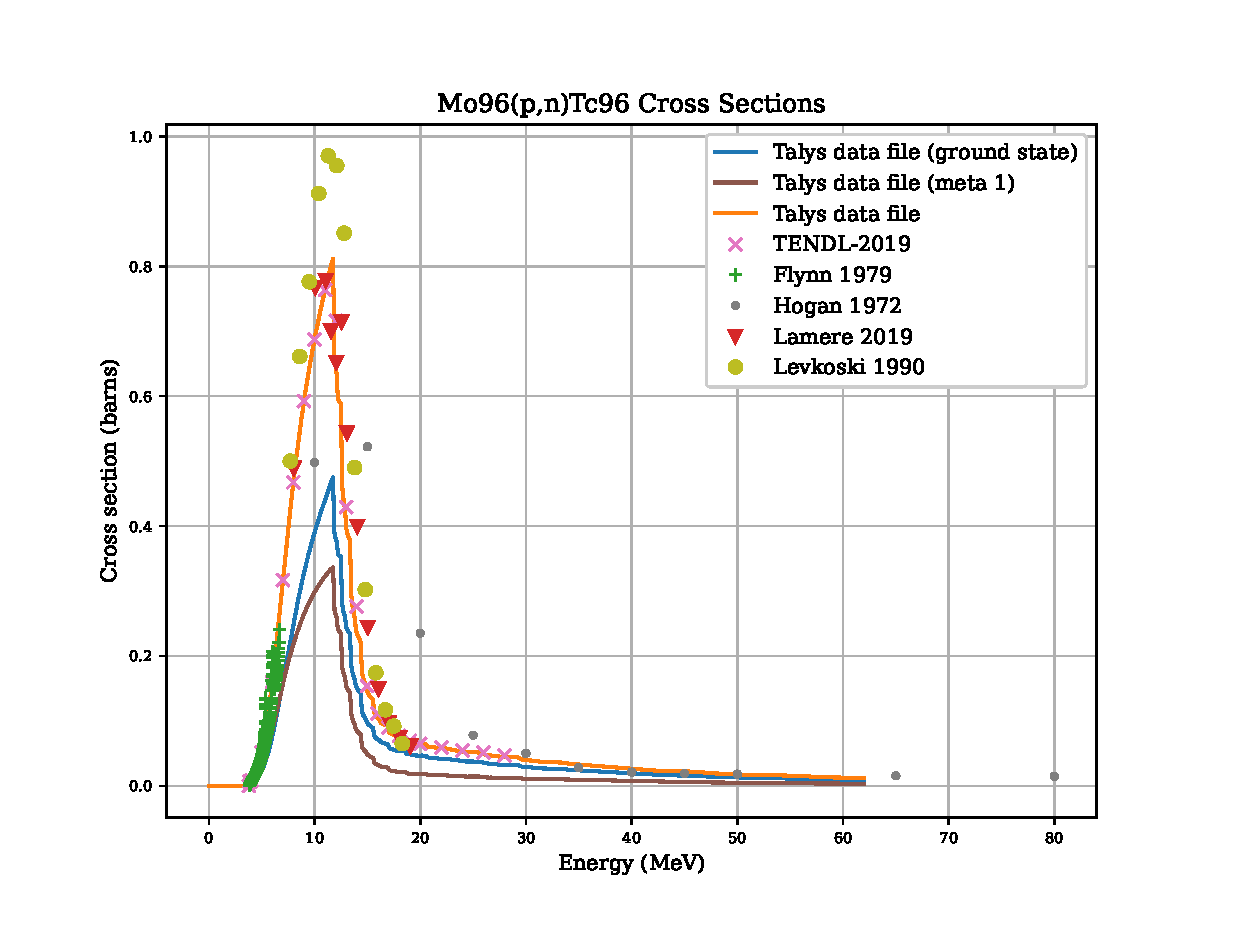
\includegraphics[width=0.7\linewidth]{chapters/activity_code/mo96_tc96/Mo96_Tc96.eps}
\caption{Reaction cross sections for ${}^{96}_{42}Mo (p, n) {}^{96}_{43}Tc$ from various sources}
\label{fig:mo96tc96xs}
\end{figure}

The cross sections computed by the TALYS code are split into both the reaction to the Technetium-96 ground state and metastable 1 state.  The separate data are plotted in figure \ref{fig:mo96tc96xs} along with their combined cross section.  

This estimate will calculate the contribution from the ground state only.  The metastable state of ${}^{96}_{43}Tc$ has a 2\% chance to decay directly to ${}^{96}_{42}Mo$ and a 98\% chance to decay to the ground state.  The half life for the metastable state is 51.5 minutes\cite{jeff311} and, coupled with a lower reaction cross section than the ground state, it will contribute a relatively small amount of ${}^{96}_{43}Tc$ when compared to those created by the ion beam and will delay the production of the ground state past the point at which the beam is removed.

The 13MeV protons will lose all their energy within the first 375 micrometers of the material as computed by SRIM (figure \ref{fig:stoppingdistanceprotons}).  As the ions lose energy the probability of a reaction occurring changes.  The cross section ranges from a maximum of 475mb at 11MeV and this drops to zero once the ion energy falls to 3.8MeV.  The average cross section over the entire energy range based on SRIM stopping distance calculations and TALYS data is 0.269 barns.

Given the data used is in good agreement with \acrshort{exfor} experimental data, the 13MeV is expected to transmute $2.93 \times 10^9$ ${}^{96}_{42}Mo$ atoms into ${}^{96}_{43}Tc$ every second.  By the end of the beam almost $4.4 \times 10^{12}$ atoms will have been transmuted via this reaction and, as the half life of ${}^{96}_{43}Tc$ is 247 times greater than the 1,500s beam duration, atoms lost to decay during irradiation will be ignored in this estimate. The intensity of each gamma varies, and these are listed in \ref{table:johnhewettresults}.

\begin{table}[h]
\begin{center}
\begin{tabular}{c c c c c}
\hline\hline
Peak & Energy (KeV) & Measured Activity (Bq) & Estimated Activity (Bq) & Factor of Over Estimate\\
\hline\hline
2 & 778 & $1.355 \times 10^{6}$ & $4.74 \times 10^{6}$ & 3.5\\
3 & 813 & $1.155 \times 10^{6}$ & $4.15 \times 10^{6}$ & 3.6\\
4 & 850 & $1.386 \times 10^{6}$ & $4.93 \times 10^{6}$ & 3.6 \\
5 & 1127 & $2.103 \times 10^{5}$ & $7.66 \times 10^{5}$ & 3.6 \\
\hline\hline
\end{tabular}
\end{center}
\caption{A comparison between measured and estimated peaks from a 0.5mm thick sample of Molybdenum irradiated with 13MeV protons at 5 microamps for 1,500 seconds}
\label{table:johnhewettresultsvestimate}
\end{table}

There is a discrepancy between the measured amount and that predicted by past work, and it is consistent across the four gamma peaks.  There are several simplifications with this estimate including the omission of the metastable state, but the inclusion of this would increase the estimated activity rather than decrease it.

My colleague investigated the affect of self attenuation of gammas passing through the Molybdenum sample.  They made the assumption that the radioactive isotopes were concentrated half way through the thickness of the sample and that the gammas would need to pass through 250 micrometers of matter.  It was expected that gammas above 200KeV would retain 94\% of their intensity with those above 1MeV having 98.5\% of their original intensity\cite{johnhewett}.

The distribution of radioactive isotopes would in fact be closer to the surface of the material than the midway point.  This is illustrated in figure \ref{fig:mo96tc96activitydepth} and it shows the majority of the Technetium-96 is created in the top 150 microns.  This plot is based on the SRIM stopping range for protons in Molybdenum and the cross section data used in the estimate.

\begin{figure}[htb]
\centering
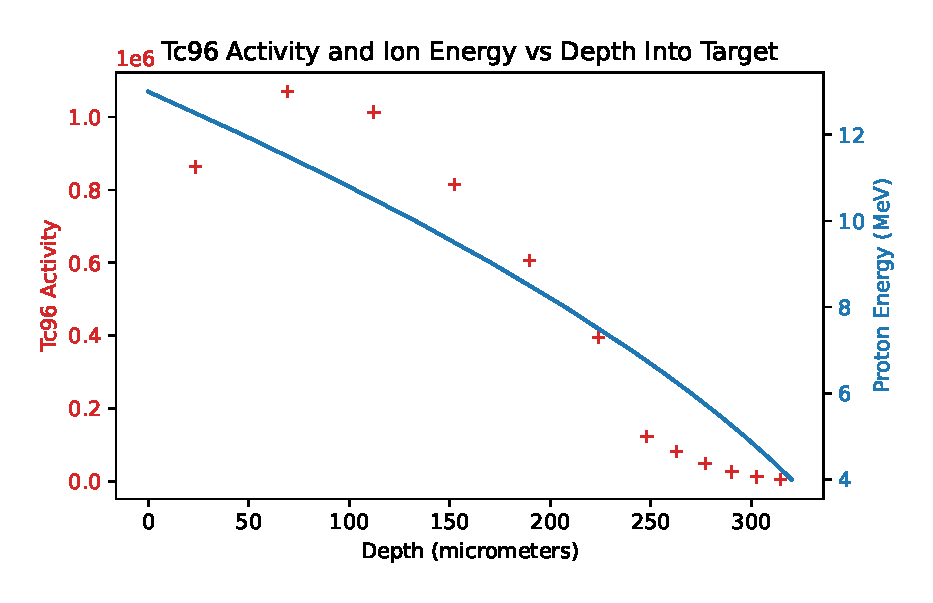
\includegraphics[width=0.7\linewidth]{chapters/activity_code/mo-john-hewett/mo96_pn_tc96_activity_depth.eps}
\caption{Technetium activity and beam energy as a function of depth into the target, showing a non-uniform distribution of radioactive atoms in the sample}
\label{fig:mo96tc96activitydepth}
\end{figure}

It is plausible that the orientation of the sample would affect the gamma count.  If it were placed such that the beam irradiated side faced the detector there would be less material between the radiation source and the detector.  The opposite way round and more material would block the path of the gammas to the detector, thus decreasing their intensity.

\begin{figure}[htb]
\centering
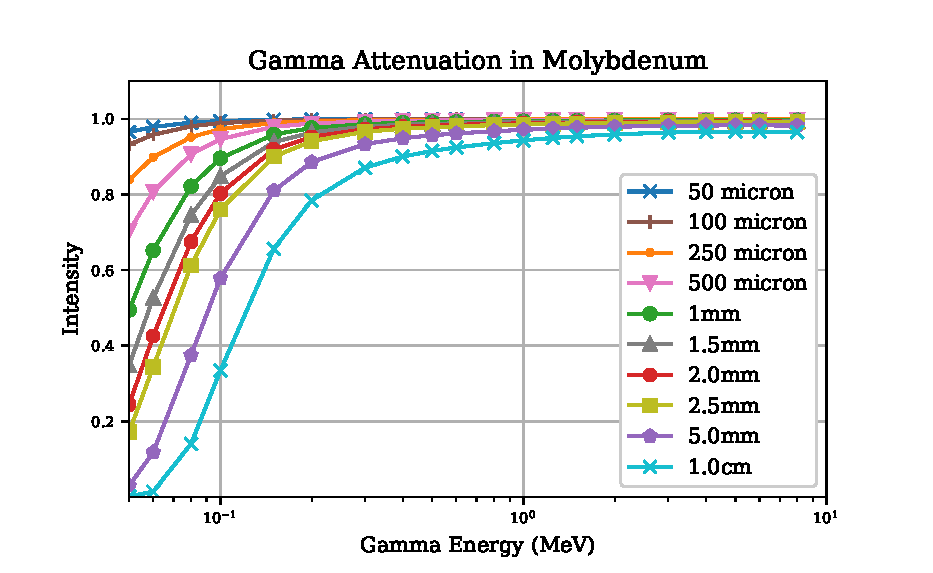
\includegraphics[width=0.7\linewidth]{chapters/activity_code/mo-john-hewett/attenuation/mo_gamma_attenuation.eps}
\caption{The attenuation of Gammas through Molybdenum for a range of energies and thicknesses\cite{massattenuation}}
\label{fig:moattenuation}
\end{figure}

When plotting the gamma attenuation through Molybdenum over a range of gamma energies it is clear that those with an energy of 500KeV or more are drop to an intensity of as low as 0.9 in targets up to 1mm thick (figure \ref{fig:moattenuation})\cite{massattenuation}.  This is double the target depth of the thick target and so it does not explain the discrepancy between the experimental and estimated values.



\subsection{Simulated Proton Irradiated Molybdenum}

Both the thin and thick samples irradiated experimentally are simulated.  However, detailed data are available for the thick sample only.  A qualitative comparison of the thin sample will be made with the experimental results available.

Only stable isotopes are included in the cross section data file currently and, as 3 out of the 7 ``stable'' isotopes are either observationally stable, or have an incredibly long half life, their reactions are not included.  The addition of these isotopes could highlight additional reactions but the data would need to be created first, if possible, using TALYS.

Out of the four stable isotopes of Molybdenum, ${}^{96}_{42}Mo$ is responsible for most of the radioactivity both at the time the beam is turned off (1,500s) (figure \ref{fig:motargetisotopes1500s}) and after 3 days of cooling (figure \ref{fig:motargetisotopes3days}).  As discussed earlier this is due to the creation of both the ground state and metastable 1 state for Technetium-96.  Whilst the beam is on over 60\% of the activity is due to the metastable-1 isotope.  The gamma energy emitted by the isomeric transition is comparatively low with an energy of just 32.28keV, and as a result it's contribution to the power output is also low.  In contrast the transition to the ground state for ${}^{96}_{43}Tc$ (meta 1) releases many energetic gammas.  The majority of the energy released towards the end of the ion irradiation is due to both the ground state and metastable 1 of Technetium-94 (figure \ref{fig:moresidualenergy1500s}).

After three days of cooling the almost 67\% of the decays are due to the ground state Technetium-96 isotopes in the sample with another 31\% from Technetium-95 (figure \ref{fig:moresidualisotopes3days}).  The gamma energy output is also primarily due to these two isotopes, although with an 87\% and 12\% split (figure \ref{fig:moresidualenergy3days}). 

\begin{figure}[htb]
\centering
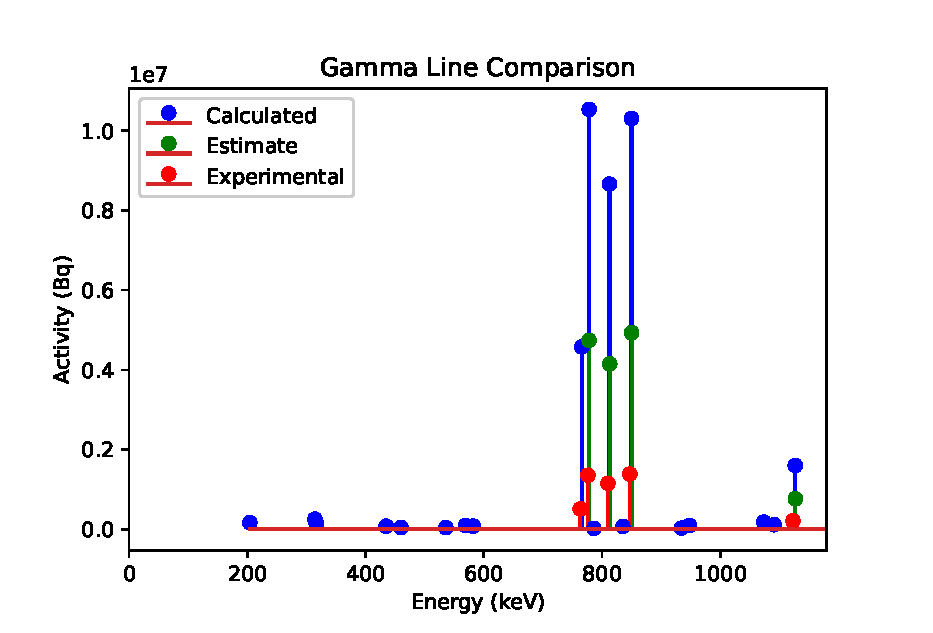
\includegraphics[width=0.5\linewidth]{chapters/activity_code/mo-john-hewett/thick/plot_gammas/gammas.eps}
\caption{Comparison of Gamma peaks from experiment, a simple estimate and the Activity code.}
\label{fig:mogammacomparison}
\end{figure}

It is clear that there is a disagreement in the values of the experimental, estimated and computed activities and gamma lines.  The fact that the estimated activities are lower than the calculated values was expected as the estimate only considered one reaction.  The difference between the experimental work with both the estimated and calculated values is harder to explain but will be discussed in section \ref{}.  The full results from the activity code are included in appendix \ref{appendix:johnmo}.


\begin{table}[h]
\begin{center}
\begin{tabular}{c c c c c}
\hline\hline
Peak & Energy (KeV) & Measured Activity (Bq) & Computed Activity (Bq) & Factor of Over Estimate\\
\hline\hline
1 & 766 & $5.118 \times 10^{5}$ & $4.574 \times 10^{6}$ & 8.9\\
2 & 778 & $1.355 \times 10^{6}$ & $1.053 \times 10^{7}$ & 7.8\\
3 & 813 & $1.155 \times 10^{6}$ & $8.658 \times 10^{6}$ & 7.5\\
4 & 850 & $1.386 \times 10^{6}$ & $1.030 \times 10^{7}$ & 7.4 \\
5 & 1127 & $2.103 \times 10^{5}$ & $1.601 \times 10^{6}$ & 7.6 \\
\hline\hline
\end{tabular}
\end{center}
\caption{A comparison between measured and calculated peaks from a 0.5mm thick sample of Molybdenum irradiated with 13MeV protons at 5 microamps for 1,500 seconds}
\label{table:johnhewettresultsvcalculated}
\end{table}





\FloatBarrier
\section{Proton Irradiated Molybdenum Doped Steel}

Another colleague in the Metallurgy and Materials department at the University of Birmingham, Alex Dickinson-Lomas,  requested a copy of the Activity code and a simulation of a steel with a specific composition (Fe: 96.375, C: 0.772, Cu: 0.024, Mn: 1.36, Ni: 0.698, Si: 0.381, Cr: 0.092, V: 0.008, P: 0.009, S: 0.003, Mo: 0.278) that would be irradiated with 5MeV protons.

In comparison to the previous cases, 36MeV protons in Iron and 13MeV protons in Molybdenum, the activity is much lower.  The simulated beam current was 0.5 microamps and the duration 5 minutes, but in contrast to the 100MBq maximum activity of the Iron sample, this is expected to reach a maximum of just over 10KBq with a gamma output of just $1.0 \times 10^{-8}$mW.

During irradiation, the isotope responsible for the majority of the residual radioactivity is ${}^{13}_{7}N$ and this is created through the ${}^{13}_{6}C(p, n){}^{13}_{7}N$ reaction.  This is despite the stable isotope carbon-13 having a percentage by mass in the sample of 0.008322\%.

The reaction probability for ${}^{13}_{6}C(p, n){}^{13}_{7}N$ is also high in the 4-5MeV range with a cross section between 0.1 and 0.15 barns.  In contrast the first reaction of note for Carbon-12 results in Boron-9 and this begins at proton energies near to and above 10MeV.

After a day of cooling the activity due to Nitrogen-13 will have decayed through 144 half lives to nothing.  The reaction responsible for almost 40\% the radioactivity at this point is predicted to be ${}^{58}_{26}Fe(p, n){}^{58}_{27}Co (meta 1)$.  Other residual isotopes of note are ${}^{57}_{27}Co$, ${}^{58}_{27}Co$, ${}^{55}_{26}Fe$ and ${}^{55}_{27}Co$.  A full breakdown is included in appendix (\ref{appendix:alexsteel}).

Whilst there are no experimental activity data to compare to, the Activity code is a useful tool.  It takes a complex material and highlights likely reaction interactions, highly radioactive residual isotopes and gamma peaks.  It also predicts the total activity expected and the calculation may be run multiple times with a range of target thicknesses and beam energies.


















